\chapter{范式简介}
\label{chap:machine-learning-paradigms}

第~\ref{chap:introduction}章的做法是：先让模型对训练邮件作出预测，再用已知标签给预测打分，并据此调整模型。它隐含一个前提——每封训练邮件都有可靠的类别，而现实中这个前提常常不成立：多数邮件可能根本没有标注；下棋或控制机器人时，更不可能为每种处境预先写出正确动作，系统只能看到一个动作之后发生了什么；长期运行的系统还会不断遇到新数据、新任务，数据也可能分散在不同设备上。于是本章要回答三个问题：标签很少时还能怎样学习？只有行动后果可观察时怎样学习？数据和任务随时间变化时，已有知识又怎样保留和复用？回答它们，关键是弄清经验以什么方式进入学习。

为此先要区分\term{学习范式}（learning paradigm）：它规定学习时可以利用哪些经验、反馈从哪里来，以及学习过程怎样组织。任务、模型与范式各管一件事：任务规定要完成什么，模型用某种形式表达输入与输出之间可能的规律，范式则规定凭什么经验、什么反馈去学到这些规律。表~\ref{tab:task-paradigm-model}继续用垃圾邮件系统对照这三个层次。

\begin{table*}[htbp]
  \centering
  \small
  \begin{tabularx}{\linewidth}{@{}lXXX@{}}
    \toprule
    \textbf{层次} & \textbf{回答的问题} & \textbf{垃圾邮件例子} & \textbf{与其他层次的关系} \\
    \midrule
    任务 & 系统要完成什么？ & 判断一封邮件是否为垃圾邮件 & 可以更换模型，任务仍是分类 \\
    模型 & 用什么形式表示输入与输出的关系？ & 逻辑回归、决策树或神经网络 & 同一模型可以用于不同学习范式 \\
    学习范式 & 系统利用什么经验和反馈？ & 从带类别标签的历史邮件学习 & 可以更换模型，仍是监督学习 \\
    \bottomrule
  \end{tabularx}
  \caption{任务、模型和学习范式描述机器学习问题的不同层次。它们相互关联，
  但不存在固定的一一对应关系。}
  \label{tab:task-paradigm-model}
\end{table*}

同一个分类任务，可以用完整标签训练，可以把少量标签与大量无标注邮件结合，也可以先让模型从无标注文本中学到特征、再用少量标签学分类。三种做法的任务和模型完全可以相同，真正的区别只在于利用了什么经验。这里说的特征仍属于第~\ref{chap:introduction}章介绍的表示，既包括词数、链接数这类手工特征，也包括模型自己学到的特征。反过来，模型名称也说明不了范式：神经网络可以接受各种来源的反馈，“用了深度学习”并不指明任何一种范式；文本或图像生成只说明了任务是什么，同样确定不了经验和目标从哪里来。

本章就按开头的三个问题展开。先比较三种最基本的反馈来源：与输入配对的目标、数据自身的结构、行动后果带来的奖励；再讨论标签不足时怎样获取和利用额外的训练依据，数据和任务变化时怎样共享、保留和迁移已有知识；之后加入学习时序与协作环境的限制；章末用组合案例说明这些设定如何在同一个系统中配合。这些分组按问题划分，彼此并不互斥：同一个方法可能既规定反馈来源，又规定知识复用或协作方式。因此判断一个系统属于哪种范式，要逐项检查它满足的条件，而不是替它找一个唯一标签。

本章只建立最基本的区别，完整的研究地图由后续专题展开：交互决策见\BookVolumeRef{vol:reinforcement-learning}{卷7《学习范式：强化学习》}；有限标签等训练依据的取得与处理、已有知识的复用与更新共享，见\BookVolumeRef{vol:knowledge-learning}{卷8《学习范式：知识的获取、演进与迁移》}。本章的中间三节就是这些专题的入口。在线学习和联邦学习只分别限定更新时序和协作环境，可以叠加在上述任何范式上，因此不为它们单列专题部分。

\section{监督学习}
\label{sec:supervised-learning}

先看最熟悉的情形：已有一批邮件，而且每封都知道类别。训练时先让模型预测，再拿已知类别对照结果、调整模型。这种利用“输入—目标”配对示例学习预测关系的方式，称为\term{监督学习}（supervised learning）。每个配对示例同时起两个作用：目标告诉我们希望模型输出什么，预测与目标的差距则为调整模型提供依据。学好的关系随后用于从未见过的新输入——那时不再有目标可用。

目标的具体形式随任务而变：分类预测类别，回归预测数值（如成交价），机器翻译预测对应的译文，还可以预测排列或其他序列。输出形式虽然不同，但都能用已有目标评价预测、并据此指导学习，所以监督学习并不只包括分类和回归。目标也不一定来自人工标注：手写数字的类别通常由人给出，房价可以直接取自成交记录，天气的“目标”可以是之后实际观测到的天气。“监督”强调的是训练示例给出了希望预测的对象，并不要求训练过程中有人实时干预。

MNIST让这一分工具体可见：数据把手写数字图像与数字类别配对，研究者据此训练并检验模型能否识别新笔迹\scite{lecun1998}。图~\ref{fig:supervised-mnist-process}中，图像送入模型以产生预测，标签单独用于比较；使用阶段只有新图像，由训练模型判断类别。

光比较出对错还不够，还要把结果变成能驱动学习的量。真实数字是“3”时，我们既可以检查模型最终选了哪个类别，也可以检查它给“3”这个类别的概率有多高；房价任务则可以衡量预测价与成交价差了多少。损失函数把任务要求翻译成这样一个可计算的数，学习算法再依据它调整模型，使预测在训练样本上越来越接近目标。算法可以千差万别，但都必须先说明怎样评价一个候选预测。

模型在训练数据上变好，并不能自动说明它在新输入上也好，这一点必须单独检查。做法是留出一批测试样本：它们的标签在训练和调参阶段都不能使用，只在最后评价时对照预测。如果看着测试答案反复修改模型，选择结果便依赖这批测试样本，原分数不再是独立的泛化估计。被选模型仍可能学到可推广的关系，但不能再用参与选择的同一批答案证明这一点。

\begin{figure*}[htbp]
  \centering
  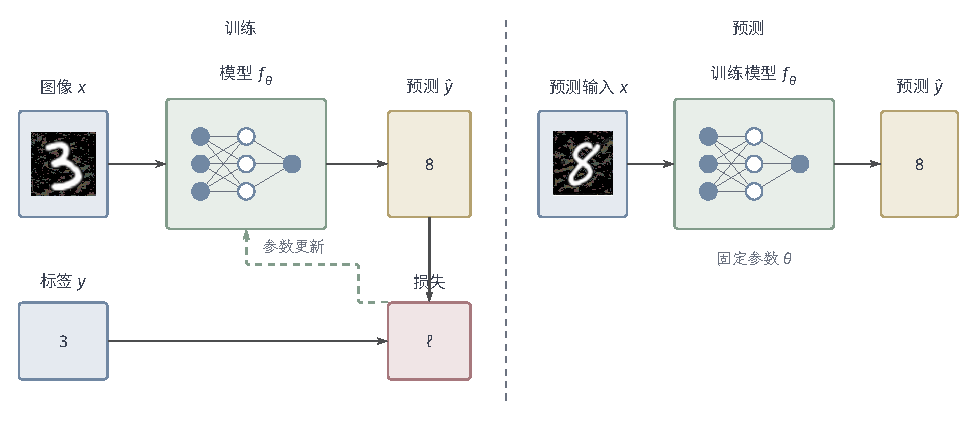
\includegraphics[width=164.600mm]{figures/03-foundations/01-basics/tikz/supervised-learning/figure.pdf}
  \caption{监督学习中的训练与预测。训练时图像进入模型，目标标签单独进入损失比较，虚线反馈用于更新参数；使用时只提供新图像。训练行中，数字3被暂时预测为8，原标签3只进入比较；使用行没有提供目标。数字字形为教学构造，不是MNIST原始样本；模型框不指定网络架构。}
  \label{fig:supervised-mnist-process}
\end{figure*}

既然监督学习的依据就是这些配对示例，它能学到什么，也受两件事限制：目标是否可靠，样本覆盖是否充分。先看覆盖。某种书写风格从未在训练集中出现时，模型也许能借助与已见数字共有的笔画识别它，但这只是可能；训练集和测试集上的成绩都没有包含这种风格，无法为它作保。再看可靠性。如果标注者习惯把某种写法的“7”标成“1”，模型会把这种错误当作规律学进去，而用同一批标签计算的分数也看不出问题，只能另找可靠的核验依据。

这两种缺口都不能靠重复训练弥补：同一批记录多训练几轮，样本的覆盖范围和标签的正确与否都没有改变。同样，数据集的名字也不能保证训练时学到的输入—目标关系在真实应用中继续成立，例如用扫描表格训练的识别器能否处理手机拍摄的数字，需要在手机照片上另行检验。标签规定了希望模型预测什么，而一份有限的标签集合未必涵盖将来出现的所有情况。

\section{无监督学习}
\label{sec:unsupervised-learning}

再考虑没有任何逐样本答案的情形：面对一批新闻，我们仍然可以观察哪些词经常一起出现、哪些文档内容相近，并用这些规律把内容组织起来。这种不依赖逐样本目标、直接从数据中发现结构或分布的设定，称为\term{无监督学习}（unsupervised learning）。

要寻找的规律由用途决定。\term{聚类}（clustering）依照相似性形成群组，可用于探索购买行为；\term{降维}（dimensionality reduction）以较少变量保留重要变化或邻近关系，可服务于可视化、压缩和后续分析；\term{分布建模}（distribution modeling）描述观测出现的规律，可用于采样或识别不常见观测。没有标签并不妨碍设定这些目标，只是检查依据转向了数据及所作假设。

顾客聚类说明表示怎样影响发现的结构。只比较购买金额，群组可能主要区分消费水平；加入购买时间与商品种类，就可能反映不同购物习惯。算法可以反复调整分组，让组内样本在选定表示下更相似，但最终分组始终依赖所用特征与相似性标准。省去答案以后，学习目标和假设仍然存在。

聚类给每条记录分配一个群组，这对新闻并不总是合适。一篇新闻可能同时涉及体育和经济，硬把它归入唯一一个群组会丢掉这种混合成分。主题发现要回答的因此不是“这篇新闻属于哪个给定类别”，而是“这批新闻里隐含着哪些主题，每篇新闻由哪些主题按什么比例组成”。没有人事先给出主题清单；模型只观察同一篇文档中哪些词倾向于共同出现。例如“进球”“球队”“联赛”常在同一批文档中出现，“利率”“股市”“通胀”常在另一批文档中出现，模型就可能归纳出两个主题，再把一篇谈论球队上市融资的新闻表示为两者的混合。主题的含义则由人看到代表词之后再解释和命名。

潜在狄利克雷分配（latent Dirichlet allocation, LDA）是实现这种思想的一种具体模型。它把每个主题表示为词汇表上的一个概率分布：高概率的词就是该主题的代表词；每篇文档则对应一组主题比例。原始研究在16{,}000篇TREC AP新闻上归纳出100个主题\scite{blei2003}。需要注意，词汇表是预先确定的观测范围，模型学习的是其上的主题词概率与文档主题比例，而不是连词汇表一起学出来。图~\ref{fig:unsupervised-topic-process}展示了这一过程：整批文档提供统计规律，学好的模型再用来描述一篇新文档的主题组成。

\begin{figure*}[!htb]
  \centering
  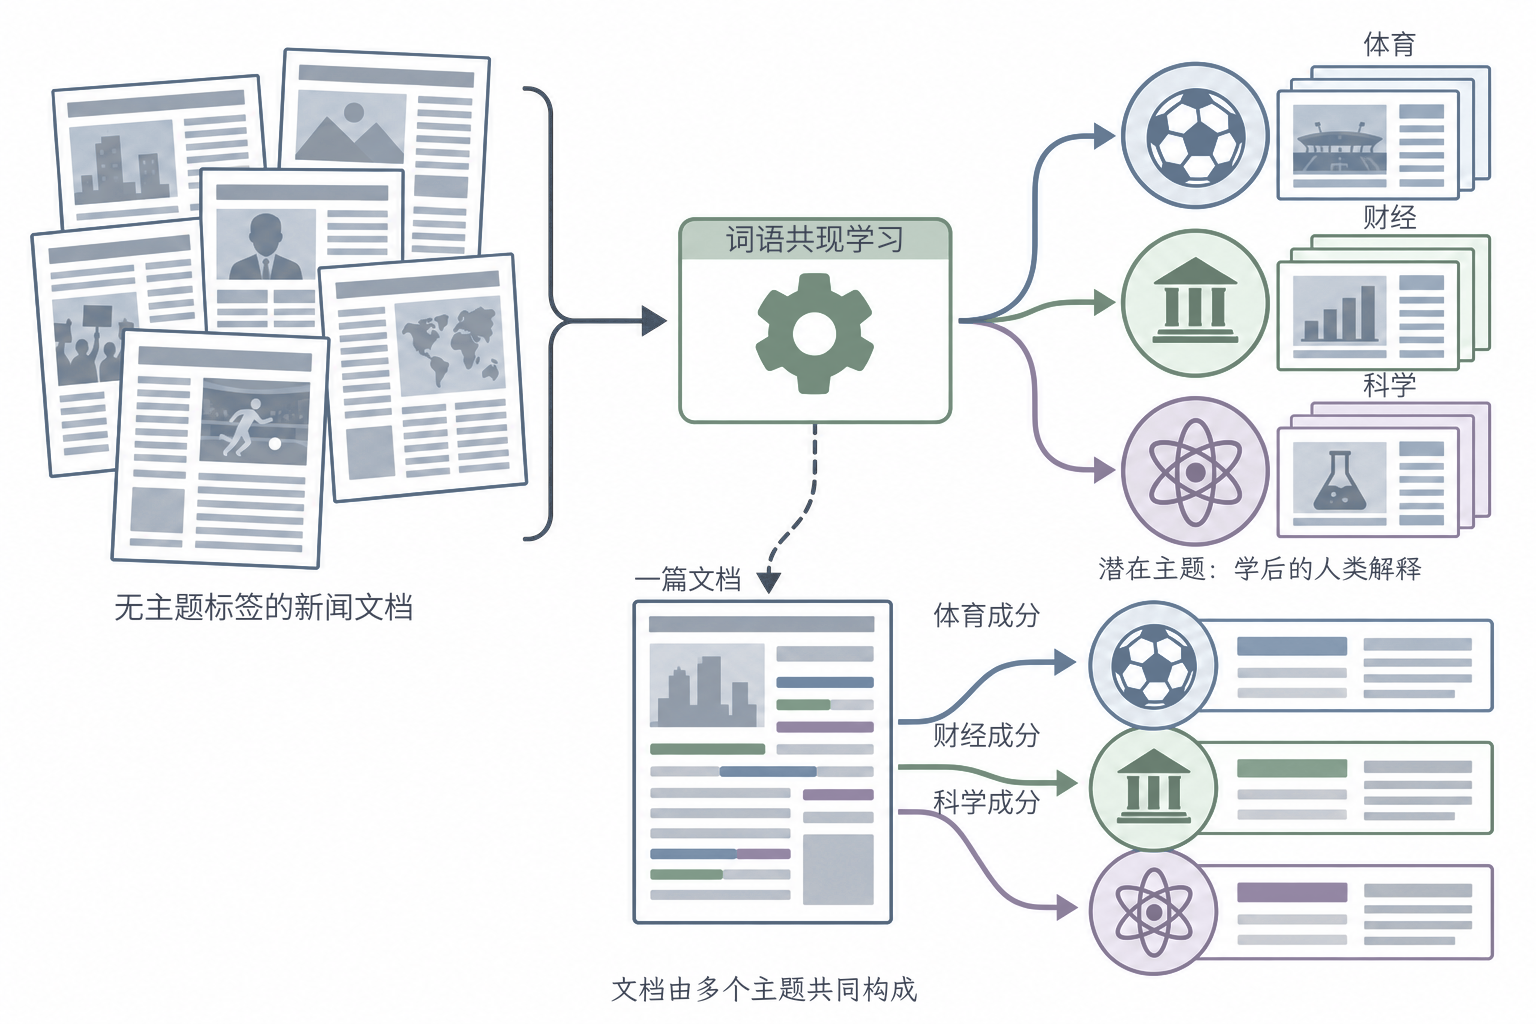
\includegraphics[width=164.600mm]{figures/03-foundations/01-basics/generated/unsupervised-topics/figure.png}
  \caption{无监督主题发现的过程示意。没有主题标签的新闻集合提供词语共现信息，学习过程形成
  若干潜在主题；同一篇文档可以由多个主题共同构成，主题名称是在结果解释阶段由人给出的。}
  \label{fig:unsupervised-topic-process}
\end{figure*}

同一份新闻数据，学习目标不同，范式也不同。如果预先规定好“体育”“财经”等类别，并给每类若干标注示例，让模型判断新文档属于哪一类，那是监督分类：类别集合和每篇文档的答案都在外部给定。主题发现没有这两样东西：主题本身是学习的产物，文档与主题的对应关系也是模型归纳的；人事后把某个主题命名为“体育”，这个名称也没有在训练中当作标签使用。区分两者的依据，是答案由外部给定还是从数据分布中归纳。

正因结构是发现而不是被告知的，无监督学习的结果必须换一种方式检验，尤其要把“算法算出的结构”和“人赋予的解释”分开。把顾客的几十项特征压缩成两个坐标后，确实可以画出图来看邻近关系，但坐标轴本身未必有“收入”或“年龄”的含义，图上分开的群组也未必是业务真正关心的人群。新闻主题至少可以从三方面检查：代表词能不能概括相关文档的内容（解释性），换一批同来源新闻后高概率词是否大体稳定（稳定性），按主题整理文档能否真正减少人工查找的时间（实际用途）。图上群组分得再开，也只是一种几何现象，单凭它证明不了结果有效。

\FloatBarrier
\section{强化学习}
\label{sec:reinforcement-learning}

前两节的例子有一个共同点：模型的预测不会改变它之后看到的数据。邮件分类器判错一封邮件，下一封邮件照样到来；主题模型怎样归纳主题，也不影响新闻库里有哪些文章。这只是前面例子采用的分析基线，并不是监督或无监督学习的定义条件，二者同样可以处理序列和在线到来的记录。第三类问题打破了这一点：模型的输出是一个动作，而动作会改变后续处境。下棋时当前落子既改变棋盘，也改变对手接下来的选择；机器人移动、车辆换道同样会改变下一刻面对的情况。此时只问“这一步预测得准不准”已经不够，还必须追踪动作在未来引发的一连串后果。

\subsection{什么是强化学习}

强化学习研究的就是这种“通过行动后果学习决策”的问题。描述它需要先分清交互中的角色。作出决策的一方称为\term{智能体}（agent），例如下棋程序或机器人控制器；与它交互的外部世界称为\term{环境}（environment），例如棋盘和对手，或机器人所在的房间。

环境在每个时刻处于某种处境，称为\term{状态}（state），如完整的棋盘局面。智能体实际能拿到的信息称为\term{观测}（observation）：棋盘可以完全看到，观测就等于状态；机器人的摄像头只看到眼前一角，观测就只是状态的一部分。智能体依据观测选择一个动作，环境随即转到新的状态，并返回一个数值评价，称为\term{奖励}（reward），例如到达目标得正分、撞墙得负分。智能体选择动作所依据的规则称为\term{策略}（policy），它可以是确定的映射，也可以给出各动作的概率。

有了这些角色，就可以说明强化学习要优化什么。一次交互按时间记录状态、动作和奖励，形成一条轨迹（trajectory）$s_0,a_0,r_1,s_1,a_1,r_2,\ldots$，其中$s_t$、$a_t$分别是第$t$步的状态和动作，$r_{t+1}$是执行$a_t$之后得到的奖励。评价一条轨迹时，把各步奖励累加成回报（return）：
\begin{equation}
  G=\sum_{t=0}^{T-1}\gamma^{t}r_{t+1},\qquad 0\leq\gamma\leq 1.
  \label{eq:rl-return-overview}
\end{equation}
这里$T$是交互的步数，$\gamma$称为\term{折扣因子}（discount factor），它调节远期奖励的权重：$\gamma<1$时越远的奖励权重越小，$\gamma=1$时各步奖励同等重要，$\gamma$接近0时智能体几乎只看眼前；交互不设终点时，通常要求$\gamma<1$，使无穷多项的和在奖励有界时保持有限。同一个策略在随机的环境中会产生不同轨迹，因此学习目标是让回报的期望$\mathbb{E}[G]$最大，这里的期望对策略与环境共同产生的随机轨迹求取。这个目标说明了强化学习与逐步打分的区别：一步奖励再高，如果把后续处境弄坏，整条轨迹的回报仍可能很低。

为便于分析，基准设定通常把问题写成马尔可夫决策过程（Markov decision process, MDP）：给定当前状态和动作后，下一状态与奖励的分布不再依赖更早的历史。这一假设让“当前状态”足以概括决策所需的过去信息。状态是否完全可见、转移规律是否已知，则是在此之上附加的信息条件（价值与优化的形式化概念可参考\BookVolumeRef{vol:mathematical-preliminaries-lower}{卷2《数学准备：概率、因果与决策》}）。

这套交互如图~\ref{fig:reinforcement-atari-process}所示：策略依据历史选择动作，环境返回后续观测与奖励，学习算法再利用这些含奖励的记录更新策略，如此循环。

\begin{figure*}[t]
  \centering
  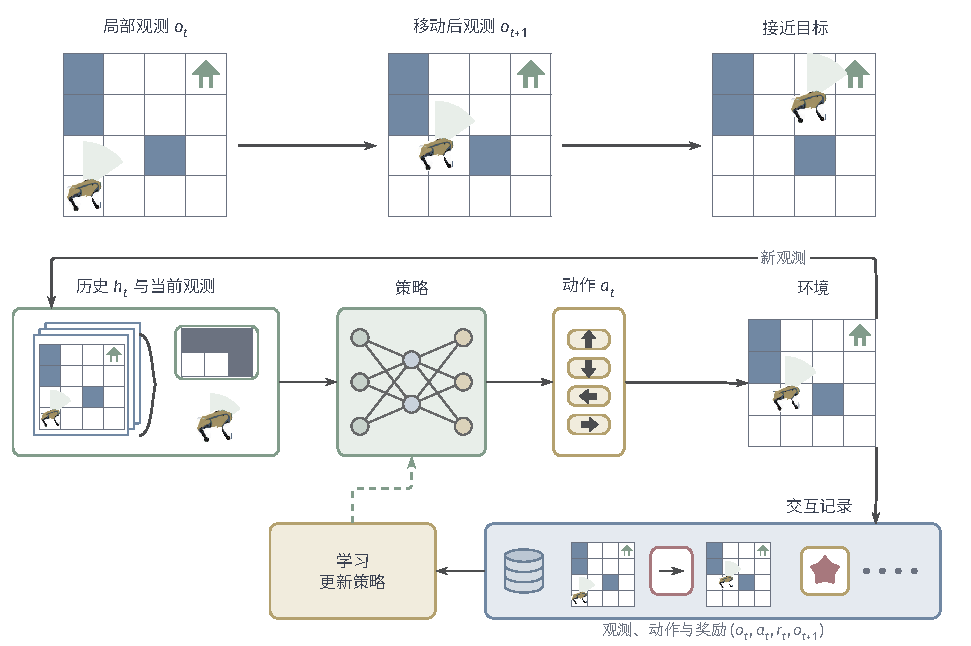
\includegraphics[width=164.600mm]{figures/03-foundations/01-basics/tikz/reinforcement-loop/figure.pdf}
  \caption{机器人探索的概念场景与强化学习的交互分工。上部导航示意展示局部观测、移动与接近目标，不表示测量结果或精确状态转移，也没有展示回合终止。下部路径表示策略、环境和学习之间的分工：策略依据历史选择动作，学习利用含奖励的交互记录更新策略；非终止时继续交互。奖励不是正确动作标签。}
  \label{fig:reinforcement-atari-process}
\end{figure*}

奖励在这套机制中扮演核心角色，但它和监督学习的标签有两点本质不同。第一，标签直接告诉模型“应该输出什么”，奖励通常只评价“刚才那个动作结果如何”，并不指出正确动作是什么。第二，反馈可能严重延迟：围棋的胜负要到终局才知道，当前多吃几个子并不保证最终获胜。因此智能体必须学会把当前选择与很久以后的结果联系起来，而不能把眼前得分直接当作长期目标。

\subsection{与监督学习、无监督学习的区别}

把三种基本范式放在一起对照，可以更清楚地看到强化学习的特殊之处，见表~\ref{tab:paradigm-comparison-rl}。

\begin{table}[htbp]
  \centering
  \small
  \begin{tabularx}{\linewidth}{@{}lXXX@{}}
    \toprule
    & \textbf{反馈是什么} & \textbf{数据怎样产生} & \textbf{学习目标} \\
    \midrule
    监督学习 & 每个输入配对的正确目标 & 本节基线使用预先给定的样本，也可扩展到序列或在线反馈 & 让预测接近给定目标 \\
    无监督学习 & 没有逐样本答案 & 本节基线分析固定记录，也可处理流式记录 & 发现数据中的结构或分布 \\
    强化学习 & 针对动作后果的、常延迟的标量奖励 & 智能体的动作改变后续状态，数据在交互中产生 & 最大化长期累计回报 \\
    \bottomrule
  \end{tabularx}
  \caption{三种基本学习范式的对照。表中样本来源采用本节基线，固定或流式不是范式判据；强化学习用奖励评价行动后果，在线交互时策略还会改变后续经验来源。}
  \label{tab:paradigm-comparison-rl}
\end{table}

与前面提供配对目标的监督设定相比，这里的强化学习不直接提供正确动作标签，而是用动作之后的奖励评价后果；在线交互时，行动还会改变后续经验来源——今天选择探索未知区域，明天面对的数据分布就随之改变，学到的策略影响它自己将来能看到什么。与无监督学习相比，虽然两者都不依赖逐样本标签，但无监督学习的目标是描述记录中的结构或分布，并不由此规定记录必须一次固定给齐；强化学习面对的是主动决策，奖励信号明确针对“行动带来的后果”，并服务于“以后该怎么行动”。所以模型连续输出动作、甚至带一些随机性，都不足以判定为强化学习；关键判据是训练是否利用动作后果的奖励、是否以长期回报为目标。

\subsection{强化学习的主要设定}

同一个强化学习问题，还会因环境信息、经验来源和行动空间结构的不同而采用不同设定。

\paragraph{环境模型是否已知：有模型与无模型}

真实交互往往昂贵：机器人每试一次都要耗时，失败还可能损坏设备。如果智能体掌握（或能从数据学到）一个\term{环境模型}（environment model），即能够预测“某状态下采取某动作后，下一状态和奖励如何分布”的模型，它就可以在真正行动前先推演几条候选路径、比较后果再决策。这种做法称为有模型（model-based）强化学习，在模型中推演并比较行动方案的步骤称为规划。模型足够可信、规划成本可接受时，推演可以替代部分真实交互；若模型与真实环境不符或难以学准，按模型选出的动作在真实环境中未必好，这一收益就可能消失。

不使用显式环境模型、直接从交互经验中学习的方法称为无模型（model-free）强化学习。它有两条常见路线。价值方法先估计“处在某状态、或在某状态采取某动作，长远来看能得到多少回报”，再选择估计值最高的动作，深度Q网络（DQN）是其代表；策略方法则不经过这一估计，直接沿着提高回报的方向调整策略本身。\term{行动者—评论家}（actor--critic）方法把两者结合：“行动者”是策略，“评论家”是价值估计，后者评价前者的动作好坏，以指导策略更新。无模型方法省去了环境建模，但需要多少交互仍取决于任务、表示和学习算法。比较两类方法的样本效率时，应固定评价目标，并计入模型学习与规划的成本；具体算法在卷七展开。

\paragraph{经验从哪里来：在线与离线}

在线强化学习边与环境交互边学习：当前策略产生经验，经验又更新策略，更新后的策略改变下一轮经历。这带来一个无法回避的矛盾——总是重复已知有效的动作（利用），可能与更优选择擦肩而过；不断尝试没把握的动作（探索），又会牺牲已有收益，这就是探索与利用的权衡。当真实交互代价高昂或有风险时，可以改用\term{离线强化学习}（offline reinforcement learning）：完全使用已经收集好的交互记录学习，训练中不再与环境发生新的交互\scite{levine2020offline}。离线方式避免了真实试错，但历史记录可能缺少将来重要的状态和动作，学到的策略在这些记录之外行动时并不可靠。与在线、离线相关的另一项区分，是更新所用经验由谁产生：只用当前策略自己产生的经验更新，称为同策略（on-policy）；允许使用旧策略、其他策略或人类操作留下的经验，称为异策略（off-policy）。离线强化学习的记录通常由其他策略产生，又不能补充新经验，常被看作异策略中最受限的情形。

\paragraph{动作是否影响未来：序贯决策与老虎机}

如果动作只影响即时奖励、不改变环境状态，问题就退化为更简单的\term{多臂老虎机问题}（multi-armed bandit）：反复在若干选项中选择并积累奖励，核心矛盾只剩探索与利用；选择时还能看到用户特征和候选内容等上下文的，称为\term{上下文老虎机问题}（contextual bandit），Li等人的新闻推荐研究即采用这一设定\scite{li2010bandit}。一旦当前推荐会改变用户未来的兴趣，动作就开始影响未来状态，必须扩展回完整的序贯决策模型。可见应用名称不决定设定，关键是哪些行动后果被纳入了评价。

\subsection{应用场景}

强化学习适用于“要做一系列决策、且后果会随时间累积”的场景。游戏是最规整的试验场：2015年的DQN用同一套算法和模型结构，仅凭游戏画面和分数就在49款Atari游戏上学会操作\scite{mnih2015}；围棋程序则通过自我对弈、按终局胜负持续改进（AlphaGo如何把人类棋谱的监督学习与自我对弈的强化学习组合，见第~\ref{sec:combining-learning-paradigms}节）。机器人用奖励衡量抓取是否稳固、是否到达目标、动作是否平稳；自动驾驶的跟车、换道和规划要兼顾安全、效率与舒适；推荐、广告竞价、调度和能源管理则在序贯决策框架下优化长期收益。是否采用强化学习，应依据“反馈是不是动作的后果、目标是否具有长期性”判断：只评价单次展示后的点击、不建模兴趣演化时，上下文老虎机通常已经够用。

\subsection{强化学习的挑战}

强化学习不需要逐步的正确动作，这使它能处理监督学习难以覆盖的决策问题，但也带来几类特有的困难。

第一类是信用分配（credit assignment）：一局棋输了，问题出在一百多步中的哪几步？奖励只在终局给出时，学习算法必须把这一个数值分摊到之前的许多动作上，而每个动作得到的信号都很微弱。

第二类来自经验本身的成本。好策略往往需要大量交互，探索又意味着要尝试没把握的动作；在真实场景中，失败可能损坏设备、无法重来。常见的缓解办法有使用离线记录、先在模拟器中训练、用专家示范建立初始行为，但它们各自引入新问题：模拟器与真实环境不符时，模拟中学到的策略可能失效；示范覆盖不足时，智能体仍会遇到没人示范过的处境。

第三类是奖励设计。真实任务往往难以写成一个数值奖励：只奖励“搬得快”，智能体就可能学会粗暴搬运、损坏物体，也可能钻奖励规则的空子，以任务设计者没有预料的方式拿到高分。难以数值化的要求可以借助人对行为片段的偏好比较来构造奖励（见第~\ref{sec:combining-learning-paradigms}节），但奖励分数提高不等于任务真正完成，最终仍要按真实要求检验。

专家示范还可以绕开奖励设计，直接提供行为依据，这类方法称为\term{模仿学习}（imitation learning）。最直接的做法是\term{行为克隆}（behavior cloning）：把专家的观测与动作配成输入—目标对，按监督学习训练策略。它的弱点在于，学习者的小错误会把它带到专家从未到过的处境，在那里没有示范可依，错误便逐步累积。DAgger让专家为学习者实际遇到的状态补充正确动作，使训练数据覆盖学习者自己会走到的地方\scite{ross2011}。\term{逆强化学习}（inverse reinforcement learning）则反过来从示范推断奖励函数，再据此学习策略；但同一行为往往能被多种奖励解释，例如“什么都不奖励”也与任何行为相容，因此无法从示范唯一还原真实目标\scite{ng2000irl}。

最后，训练环境与部署环境的差异、策略在分布变化下的稳定性，以及如何用有限测试给出可靠性结论，都是强化学习走向应用必须处理的问题\scite{sutton2018}。

\section{知识的获取}
\label{sec:efficient-knowledge-use-overview}

收集照片往往比请专家逐张确认物种容易得多，于是可靠的任务标签常常成为学习的瓶颈。在标注预算有限时，可以想办法让已有的少量标签发挥更大作用、利用其余没有标签的原始数据，或者优先挑选最值得标注的样本。本节关心的正是训练依据从哪里来、又如何使用。

要回答这些问题，先得承认训练依据并不只有类别标签。“这两张照片拍的是同一株花”是一种样本关系，“一株花若是玫瑰，就不会同时是郁金香”是一种约束，“遮住的词原来是什么”也能充当目标。我们把这些能够指导训练的答案、关系、约束和目标统称为训练知识。

训练知识可以来自人工、规则、模型或数据本身，但在经过核验之前，它们都只能算候选知识：数量多、模型给出的确信程度高，或某个训练目标的数值好看，都不能单独证明它可靠。知识不足也不只是“数量少”，还可能是覆盖不全、粒度不合适、内容错误或已经过时，各自需要不同的处理。

既然目的是节省标注，就要说清“节省”怎样衡量。本节所说的高效，指在达到同样的目标评价要求时减少人工任务标签，或在同样的标注预算下相对既定基线改善独立评价结果；它不承诺计算更省。比较时应分别报告任务收益，以及人工、模型调用、计算和维护各方面的成本，不能用“多了多少候选标签或样本”代替真实收益。

下面按五类方法逐一辨认它们能用的资源和训练信号：半监督、自监督、弱监督、对比学习和主动学习。它们与知识来源并不一一对应，例如主动学习向人工提问，自监督直接从数据构造目标，半监督和弱监督则常常合用多个来源；节末再讨论来自不同来源的候选知识怎样汇总与核验。

\subsection{半监督学习}
\label{sec:semi-supervised-learning}

设想商品类别已经确定，但只有少量图片完成了标注。这些标签负责规定“类别是什么意思”，其余大量无标签图片则可能补充光照、拍摄角度和背景上的变化。\term{半监督学习}（semi-supervised learning）让有标签数据和无标签数据共同服务于同一个目标任务，借助后者提供的输入分布规律来扩展学习。

无标签图片怎样才能参与训练？最直接的办法叫\term{自训练}（self-training）：先用少量有标签数据训练一个模型，再用它预测其余样本，把采纳的预测当作临时目标，这样的临时标签称为\term{伪标签}（pseudo-label）。原始标签和选中的伪标签一起进入下一轮训练，之后还可以反复重新生成。预测由此提供了一条利用额外数据的途径，但伪标签并没有因此变成真实答案。筛选伪标签常看\term{置信度}（confidence），即模型对自己预测的确信程度，分类时通常直接用预测类别的概率。但自信不代表正确：一旦高置信的预测本身是错的，反复拿它训练只会把原来的误判越加固执。因此除了筛选，还要控制伪标签在训练中的权重和影响，不能把“模型很自信”当成“标签可靠”的证据。

另一条思路不急着决定类别，而是约束模型对“同一个对象”给出一致的预测。轻微改变亮度通常不应改变动物的类别，要求图像在这类变换前后预测保持稳定，就是\term{一致性约束}（consistency regularization）。同一张原图经过不同处理得到的多个\term{视图}即使都没有标签，它们之间的预测分歧也能作为调整依据。前提是变换确实保留了任务含义：如果裁剪把动物裁掉了，还要求类别不变，反而会把模型带偏。

样本之间的相似性提供了第三条途径。\term{基于图的方法}（graph-based methods）把每个样本看成一个节点、把相似关系看成边，再让少量已知标签沿着边影响邻近的无标签节点：经典图半监督方法用有标签和无标签样本共同构图，要求相邻样本的预测彼此接近\scite{zhu2003}。聚类思路则基于另一个假设——稠密地聚在一起的样本往往属于同一类。两类方法都依赖“相似性与任务相关”：背景颜色相近，并不保证物体类别相同。

FixMatch把伪标签和一致性约束结合起来\scite{sohn2020}：先对无标签图片做一次弱变换并预测，当最大类别概率超过预设阈值时才采纳这个类别作为伪标签，再要求同一张图经过强变换后的预测与它一致。真实标签负责规定类别含义，这两条要求则把训练延伸到了没有答案的图片上。其CIFAR-10实验只揭示少量训练图片的类别，其余图片以上述方式参与。这里的“无标签”是指答案对训练隐藏：即使数据集里保存着真实类别，训练过程也不允许读取。图~\ref{fig:semi-supervised-image-process}示意两路数据如何汇入同一个分类器。

\begin{figure*}[!htb]
  \centering
  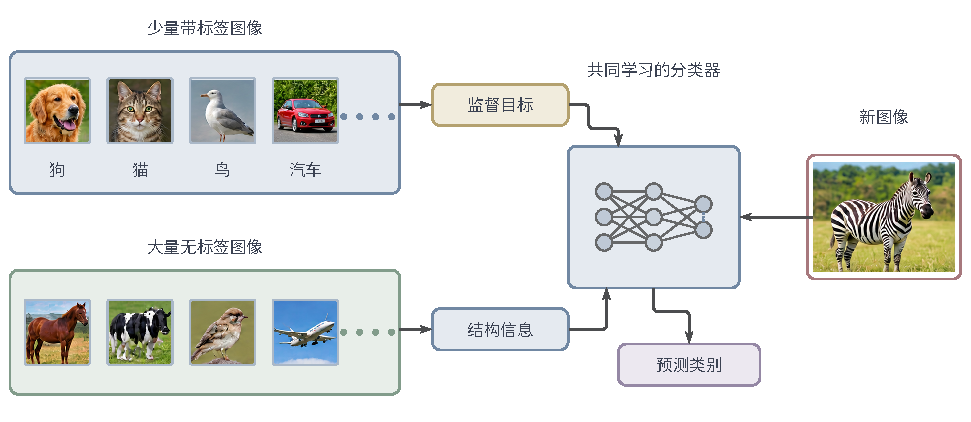
\includegraphics[width=164.600mm]{figures/03-foundations/01-basics/tikz/semi-supervised-learning/figure.pdf}
  \caption{半监督学习的过程示意。少量带类别标签的图片规定目标，大量无标签图片提供额外结构信息，两路经验共同用于形成分类能力，汇入同一分类器。模型框不指定网络结构；动物图片为教学构造。无标签图片的隐藏真值不能作为训练答案使用。}
  \label{fig:semi-supervised-image-process}
\end{figure*}

半监督还隐含一个前提：额外图片要与当前任务相关。如果加入的图片根本不属于这十个类别，模型仍可能自信地硬塞一个已知类别，再把这个错误预测当伪标签学进去。因此额外数据的适用范围必须检查——数据量增加本身并不保证有帮助。

还要说清预测的范围。如果目标是学一条能处理未来任意新输入的规则，称为\term{归纳学习}（inductive learning）；如果待预测的那批样本事先已经给定，学习只是利用它们彼此的结构为这批特定输入补全答案，则称为\term{直推学习}（transductive learning，也译转导学习），直推支持向量机采用的就是这种预先给定待分类样本的设定\scite{joachims1999transductive}。归纳与直推限定的是“哪些输入在学习时可见、评价覆盖到哪里”，半监督限定的是标签资源，二者是不同的维度，半监督完全可以采用任一种设定。直推虽然允许查看待预测输入，但它们的答案仍须隐藏；而且在这批固定输入上的表现，不能代替对未来新样本的表现。

半监督仍靠已有的类别标签规定任务。如果这些标签尚不存在，还可以从原始数据构造另一些有答案的问题，先学习日后可能复用的规律，这就是下面的自监督学习。

\subsection{自监督学习}
\label{sec:self-supervised-learning}

一份完整文本虽然没有情感标签，却天然保留着每个词。把其中一部分暂时遮住，模型就能拿“可见的上下文”当输入、“被遮住的原文”当答案——训练示例由此自动产生，无需任何人额外标注。这为标签稀缺提供了另一种训练依据。

这种直接从数据内容或关系中构造目标的方式，称为\term{自监督学习}（self-supervised learning）。遮挡内容后恢复、预测序列的后续部分、匹配同一事物的不同视图，都是常见形式。“自”限定的只是目标的来源；具体遮住什么、拿什么和什么比，仍需要精心设计。我们希望补词任务能逼模型学到语法和语义、图像恢复任务能逼它学到纹理和物体关系，但这些目标究竟带来了什么能力，仍要放到真实任务上检验。

BERT的掩码预测给出具体过程\scite{devlin2019}。文本先分成\term{词元}（token），它可以是字、词或词的一部分；训练随机选择部分词元作为预测目标，其中多数替换成掩码，另一些替换成随机词元或保留原词元，三种情况下都用原词元计算损失。原文同时提供构造输入与训练目标。例如教学句子“猫在垫子上”隐藏“垫子”后，剩余内容进入模型，原词元单独用于比较。图~\ref{fig:self-supervised-masked-process}只展示完全替换为掩码的分支；在这个教学例中，模型不能从输入读到被保留为目标的原词元。

\begin{figure*}[!tbp]
  \centering
  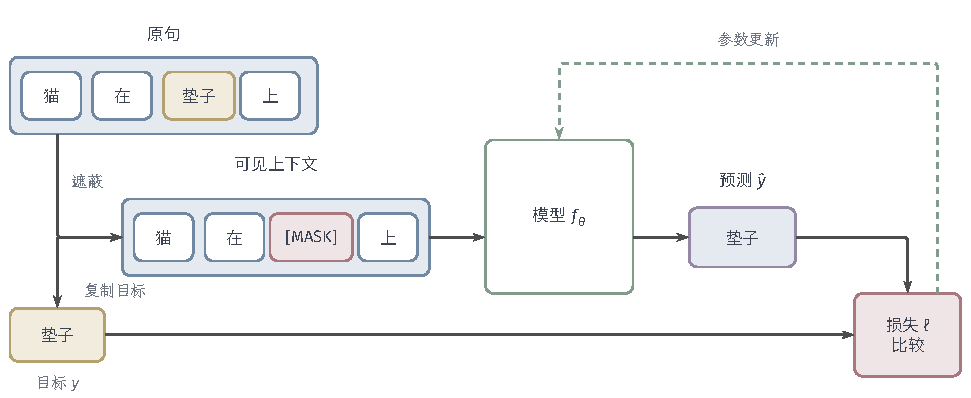
\includegraphics[width=164.600mm]{figures/03-foundations/01-basics/tikz/masked-self-supervision/figure.pdf}
  \caption{掩码预测以“猫在垫子上”为教学例子。输入将“垫子”替换为[MASK]，原词单独保留为比较目标；模型只能读可见上下文，不能读被保留的答案。可见词元共同进入模型，虚线将损失反馈到参数；模型框不指定网络结构。}
  \label{fig:self-supervised-masked-process}
\end{figure*}

构造好配对之后，就可以比较预测与答案、调整参数。“预测下一个词元”同理：只把目标词之前的文本作为输入，紧随其后的原词作为答案，因而能够批量生成训练示例。判断一个方法是不是自监督，要追溯目标是怎么来的：掩码任务的目标是恢复原文，情感分类的目标则是另外规定的评价类别；两者的区别不在于标签是否由人手工填写。

自监督与无监督学习的关系也值得说清。同一批新闻既可以做前面的主题发现，也可以做掩码预测：主题模型从词语共现中归纳潜在结构，掩码任务则把数据改造成明确的“输入—恢复目标”、逐次比较预测与答案。两者都不使用额外的人工任务标签，也都包含人为设定的目标和假设，区别并不是“有没有目标函数”。广义的无监督学习可以把自监督包含在内，因为它同样不依赖人工任务标签；本书为了讲清信号是如何构造的，把自监督单独列出，这只是内容组织上的选择，并不要求各类别互斥。

自监督目标可以直接用于文本生成，也可以分两步使用：先学一个可复用的表示，再拿它服务于分类、问答等具体任务。前一阶段称为\term{预训练}（pre-training），后一阶段要解决的具体问题称为\term{下游任务}（downstream task）。例如先让模型学习文本与上下文的关系，再用少量情感标签学评论分类，两个阶段所用目标的来源完全不同。预训练得到的规律不会自动规定下游的类别，最终任务往往仍需要标签或其他说明。构造出的目标还可能被模型“走捷径”：如果只靠局部词语搭配就能恢复遮挡词，完成这个目标未必需要理解整段文字。所以自监督到底有没有帮助，仍要以下游任务上的实际评价为准。

\subsection{弱监督学习}
\label{sec:weakly-supervised-learning}

还可以利用那些获取成本低、但质量不完善的现有标注。例如要定位图像中的汽车，手头数据可能只标注了“图中有汽车”，甚至网页标签与图片内容根本不符。\term{弱监督学习}（weakly supervised learning）研究的就是如何利用不完整、不精确或不可靠的监督，让学习不必等到所有标注都达到理想标准才开始。

一种常用划分把弱监督分成三种情况：部分样本完全没有标签，称为\emph{监督不完整}（incomplete supervision）；只有整图类别、给不出任务所需的位置等细节，称为\emph{监督不精确}（inexact supervision）；标签与内容本身不符，称为\emph{监督不准确}（inaccurate supervision）\scite{zhou2018}。第~\ref{sec:semi-supervised-learning}节的半监督主要处理第一种，属于广义弱监督；本节重点看粗粒度标签、错误标签和规则监督。

领域经验还可以先写成可批量执行的规则。Snorkel允许专家编写\term{标注函数}（labeling function）：依据关键词、文本模式或外部知识作出判断，依据不足时弃权。例如“含链接”可以提示垃圾评论，但也可能误伤正常的分享。系统综合各条规则的一致、冲突和弃权情况，估计出类别概率，再用这种概率标签训练最终模型\scite{ratner2017}。图~\ref{fig:weak-supervision-process}中的汇合，表示多条候选判断被合并成训练监督，而不是任何一条规则直接等于真值。规则也可以来自事实关联、类别约束或结构要求，产生标签、候选范围或关系判断；规则没有触发只代表“没给出判断”，不能自动当成负例。使用规则时应记录它的依据、适用对象和冲突处理方式，才说得清候选信号到底代表什么。

批量规则省去了逐条人工标注，但也会把自身的局限成批传播出去。如果多条规则都依赖“有没有链接”，即使它们结论一致，也可能一起误判正常分享；把它们当成相互独立的证据，会高估一致结论的可靠性。因此综合多来源规则时，要分别估计各自的准确性、覆盖面和相互依赖，并允许保留“不确定”的结果。规则之后再训练最终模型，本意是让模型从原始内容学到更可推广的关系、从而覆盖规则没写到的输入；但规则中的系统性偏差同样可能被模型继承。这一步是否成功，只能由独立、可靠标签上的评价决定——预测符合规则，并不能证明模型学会了目标能力。

\begin{figure*}[htbp]
  \centering
  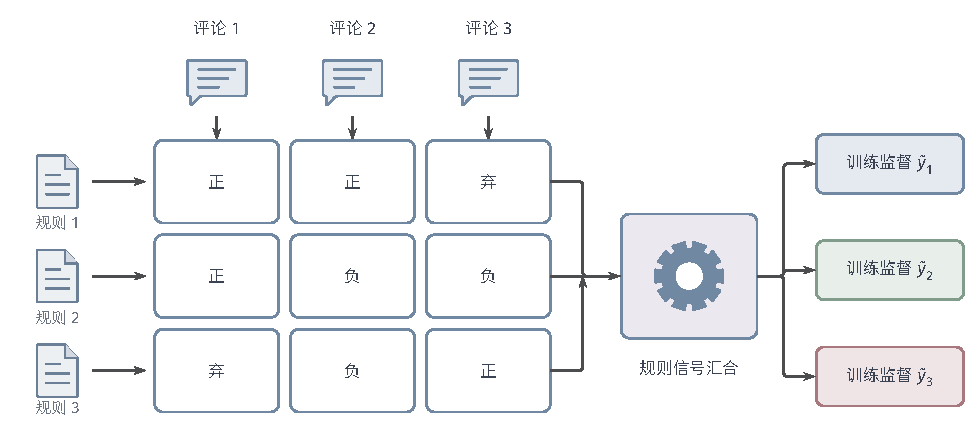
\includegraphics[width=164.600mm]{figures/03-foundations/01-basics/tikz/weak-supervision/figure.pdf}
  \caption{三条规则在三个未标注评论上的教学投票。正、负、弃分别表示两种倾向与弃票；同一列可能存在冲突。综合规则信号形成训练监督$\tilde y_i$，图中不规定合并算法，也不把某条规则输出等同于真实标签；评价仍使用独立可靠标签。}
  \label{fig:weak-supervision-process}
\end{figure*}

粗标签带来另一类困难：整图类别里缺少任务真正需要的位置信息。要从“图中有汽车”学到汽车在哪里，就要把粗监督与区域预测联系起来。可以把图像看成若干候选区域：整图有汽车只意味着“至少一个区域有汽车”，并不意味着每个区域都是汽车。这正是\term{多示例学习}（multiple-instance learning）的典型设定——监督约束施加在一组对象上，而不是逐一给出答案。如果把整图标签复制到每个区域，背景就会被错误地标成汽车。

对于\emph{带噪声标签}（noisy labels），可以识别可疑样本并削弱其影响，也可以显式建立“标签会出错”的模型，例如用少量经过核验的样本估计标注可靠性，再据此调整训练。但要注意：样本难学不等于标错了，那些少见却正确的情形同样会让模型犯错。处理弱监督的核心原则，是把已知的不确定性显式利用起来，而不是无条件把现有记录当成真值。

\subsection{对比学习}
\label{sec:contrastive-learning}

已知的对应关系也可以直接指导表示学习。同一张照片改变颜色或取景之后，“两个视图来自同一张图”这一关系仍然成立，无需任何类别标签。\term{对比学习}（contrastive learning）就用匹配与不匹配关系构造目标：使用相似度或匹配得分时，让匹配对的数值升高、不匹配对照对的数值降低；使用距离时，则缩短匹配对的距离、拉远对照对的距离。相互匹配的对象构成\term{正样本对}（positive pair），不匹配的对照构成\term{负样本对}（negative pair）。这里的“正负”只描述配对关系，不能与二分类的正负类别混淆；具体采用距离还是相似度，也要与表示的用途相符。

SimCLR先用没有提供类别标签的图片学习表示，再检验这些表示是否帮助分类。原研究在ImageNet等数据上开展这一过程，之后用标签训练分类器或调整模型\scite{chen2020}。类别标签进入评价或后续训练，并未进入前一阶段的匹配构造。

训练的具体目标，是为每张原图找到它的另一个视图。每批图片各自经过两组随机裁剪、颜色变化等变换，再由同一个模型映射成表示；同源图片的两个视图互为匹配，其他图片的视图则充当对照。为什么需要对照？如果只要求同源表示接近，模型把所有图片都映到同一个点，就能让任意两个表示完全相同，目标达到最优却什么也没学到。加入对照之后，它必须同时做到两件事：保留同一图片在变换下的联系，又区分不同图片。

这一要求可以写成一个“在一批候选中找出匹配者”的分类问题。设视图$i$的表示为$\bm{z}_i$，与它同源的另一视图记为$j$，$\operatorname{sim}(\cdot,\cdot)$是两个表示的相似度（如余弦相似度），$\kappa>0$是调节分数尖锐程度的温度系数。SimCLR类方法对视图$i$使用的损失形如
\begin{equation}
  \ell_i=-\log\frac{\exp\bigl(\operatorname{sim}(\bm{z}_i,\bm{z}_j)/\kappa\bigr)}
  {\sum_{k\neq i}\exp\bigl(\operatorname{sim}(\bm{z}_i,\bm{z}_k)/\kappa\bigr)},
  \label{eq:contrastive-loss-overview}
\end{equation}
分母对同一批中除$i$自身之外的全部视图求和，其中只有$j$是匹配者，其余都是对照。分式可以读作“在所有候选中选中$j$的概率”，最小化$\ell_i$就是提高这个概率：既要拉高分子中的匹配相似度，也要压低分母中对照的相似度。若所有表示都相同，分式等于候选数的倒数，损失并不小，这就排除了上面的投机解。

图~\ref{fig:contrastive-learning-process}用同一张鸟图的两个视图和另一张猫图作对照。模型此时并不知道“鸟”“猫”这些类别，训练信号完全来自视图的来源，所以属于自监督；反复进行这种比较，可能学到对颜色、取景等变换保持稳定的特征，但是否真的有助于分类，仍要后续检验。图中各点的位置只表示训练所要求的相对关系，并非实验测得的真实表示分布。

\begin{figure*}[htbp]
  \centering
  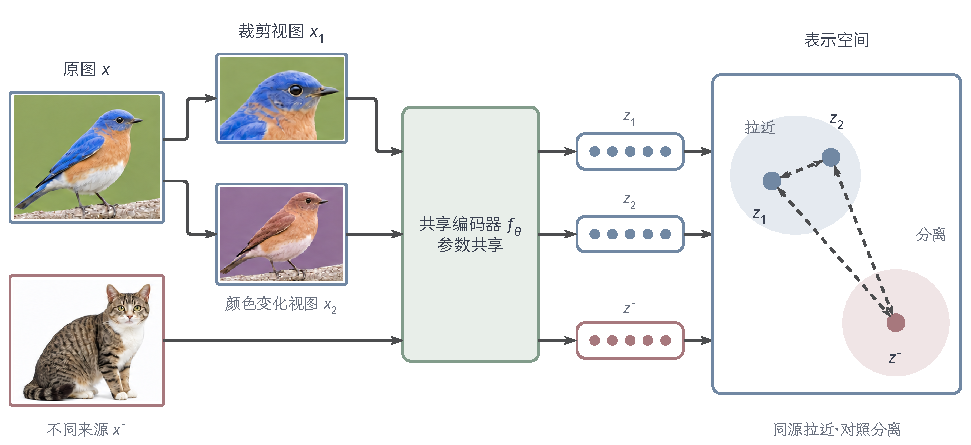
\includegraphics[width=164.600mm]{figures/03-foundations/01-basics/tikz/contrastive-learning/figure.pdf}
  \caption{自监督对比学习的教学示意。同一幅鸟的原图分别经裁剪与颜色变化形成两个视图；它们与另一幅猫图的视图经共享参数的编码器得到表示。两个蓝色点表示同源视图的表示，红色点表示其他原图的对照；箭头只示意同源拉近与对照相对分离的训练目标。动物图元和表示位置均为教学构造，不是实测影像或表示分布。}
  \label{fig:contrastive-learning-process}
\end{figure*}

匹配关系也可以由类别标签定义，此时就成为监督式对比学习\scite{khosla2020}；还可以让图像与描述它的文字互相匹配。所以“对比”限定的是目标如何构造，“自监督”限定的是信号从哪里来：SimCLR两者兼具，掩码预测用的是自监督信号但没有采用对比目标。

这些配对关系还必须服从任务含义。如果裁剪改变了图像内容，同源视图就未必还应该匹配；如果不同图片拍的是语义相近的对象，把它们一律当成负对照，反而可能妨碍后续分类。采用对比目标之前，需要想清楚哪些差别应当保留、哪些变化应当忽略。

\subsection{主动学习}
\label{sec:active-learning}

如果标签可以补充、但预算有限，第一个问题就是“先给哪些样本做标注”。\term{主动学习}（active learning）让模型根据当前已经学到的知识挑选样本，再请人或其他可靠来源提供答案，希望用有限次数的查询补足覆盖空白或纠正错误；它决定的是新增标签应该花在哪里。典型的池式设定需要四样东西：一个未标注样本池、一个当前模型、一个能可靠回答查询的来源和一笔预算。如果相关样本根本还没收集到，或者回答来源不可靠，主动选样本身补不齐缺失的信息。

Gal等人的MNIST研究从20张类别均衡的标注图开始，每轮查询10张，再学习并与随机选样等准则比较\scite{gal2017}。基准中的查询只是揭示已保存但对模型隐藏的标签，未必由现场标注者实时作答；应用中则可由医生、工程师或普通标注者提供。图~\ref{fig:active-learning-loop}展示新标签进入模型之后，下一轮选择随知识变化的循环。

\begin{figure*}[htbp]
  \centering
  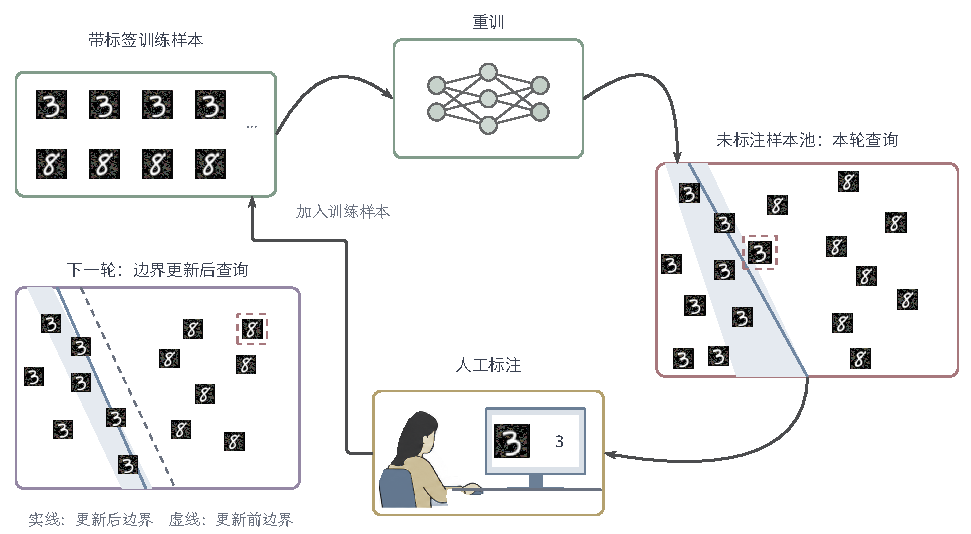
\includegraphics[width=164.600mm]{figures/03-foundations/01-basics/tikz/active-learning/figure.pdf}
  \caption{池式主动学习的教学示意。蓝色曲线表示当前模型的决策边界，红色虚线方框标出本轮查询的数字3。标注者返回标签后，样本并入带标签集合，用于重训模型。左下方的虚线保留更新前的边界，实线表示更新后的边界；虚线方框标出的数字8是下一轮查询对象。查询预算限制循环。数字字形、二维位置和边界均为教学构造，不表示实测分布或选样收益；数字样本的外观不等同于供模型使用的类别标签。}
  \label{fig:active-learning-loop}
\end{figure*}

不确定性只是选样的依据之一。一个极其模糊的数字虽然让模型很犹豫，但拿到标签后未必能提供可推广的规律；反复查询几乎一模一样的写法，得到的也多是重复信息。是否值得标注，还要综合看样本覆盖与多样性、回答的可靠程度，以及每个样本的标注成本。

主动学习可以和其他范式配合，但边界要分清。它可以和半监督一起用于数字识别：一部分样本被选中去获取真实标签，其余样本通过伪标签或一致性约束参与训练——主动学习解决“预算花在谁身上”，半监督解决“剩下的无标签输入怎么用”。

主动学习本身只决定优先询问哪些样本；答案能不能用，还取决于标注任务和判定规范、交互方式（直接作答还是候选比较）、标注者能力、复核机制和预算分配，这些都属于查询策略之外的人工知识获取环节。

“选择—反馈”的循环也不自动构成强化学习：这里查询返回的是图片标签，评价的是给定标注预算下模型在独立样本上的分类准确率；而强化学习用奖励评价动作的后果和累计回报。当然，也可以把多轮查询本身建模成序贯决策、用强化学习寻找查询策略，但那是额外的实现选择。

\subsection{标签利用方式的比较}
\label{sec:efficient-knowledge-use-comparison}

五种方法都想节省人工标签，但各自改动的是学习的不同环节。固定一个情景就能看清这一点：手上有一大批花卉照片，其中只有少量标了品种。

半监督直接围绕花卉分类，让少量标签规定类别含义，同时让其余照片通过伪标签或一致性约束参与同一任务。自监督则先不管品种，由照片自身构造目标（例如遮住一块图像再恢复）学习表示，之后仍需类别标签或其他信息来规定要识别什么。前者在目标任务内部利用两类数据，后者先为“没有任务标签”的阶段找到训练信号。

另外两种方法关心标签本身。如果专家只能给出“这是蔷薇科”之类的粗判断，或者按花色写成的规则会出错，弱监督研究怎样使用并修正这些不完善的信号；如果专家能可靠回答、但只能回答几百次，主动学习研究先问哪些照片。前者限定监督的质量，后者限定获取答案的过程，二者目的相同却不能互相替代。

对比学习与上面四者不在同一维度上：它规定的是怎样用匹配关系构造目标，而匹配关系既可以来自同源视图（此时属于自监督），也可以来自类别标签（此时属于监督）。同理，半监督处理的“部分样本无标签”也是广义弱监督中的一种。表~\ref{tab:efficient-knowledge-use-comparison}按资源、方式和条件汇总五者，用于判断一个方案需要满足哪些条件，而不是要求系统只能挑一个名称。

\begin{table*}[htbp]
  \centering
  \small
  \begin{tabularx}{\linewidth}{@{}lXXX@{}}
    \toprule
    \textbf{范式或方法} & \textbf{可以利用的资源} & \textbf{减少标签依赖的方式} & \textbf{需要检查的条件} \\
    \midrule
    半监督学习 & 少量标签与无标签数据 & 让无标签样本也参与目标任务学习 & 数据结构与目标类别是否相符 \\
    自监督学习 & 原始内容及其关系 & 从数据中构造训练目标 & 所学规律是否对实际任务有用 \\
    弱监督学习 & 粗标签、噪声标签或规则 & 接受成本较低的不完善监督 & 标签误差及不同来源的依赖 \\
    对比学习 & 视图、配对关系或类别标签 & 用匹配关系学习可复用表示 & 匹配依据是否可靠；也可使用标签 \\
    主动学习 & 可查询的样本与标注来源 & 优先为有价值的样本获取标签 & 查询收益、样本覆盖与标注成本 \\
    \bottomrule
  \end{tabularx}
  \caption{围绕有限标注比较知识的获取与使用。减少人工任务标签并不等于减少全部训练成本，
  也不保证这些方法在任意数据上都能提高效果。}
  \label{tab:efficient-knowledge-use-comparison}
\end{table*}

实际系统常常同时使用几种方法，同一张照片可能既有规则给出的粗标签，又有模型生成的伪标签，还被专家看过一眼。这些候选知识在进入训练前，需要先融合。融合前要确认它们说的是同一件事：对象是否相同（整图还是某个区域），语义是否相同（“蔷薇科”与“月季”粒度不同），然后再评估各来源的覆盖、偏差和相互依赖。融合结果可以是单个标签、类别概率、候选集合，也可以是“弃权”，不必强行给出答案；几个来源意见一致，也可能只是共享了同一个错误。标签、关系和约束如果无法化为同一语义下的判断，就应保留各自的含义分别参与训练，不能直接投票。

融合之后还要检查质量。做法是用独立依据和有代表性的抽查样本，把问题分成已确认的错误、需要复核的线索和信息不足三类，追查它们出自哪个来源或哪个构造环节，修正后再独立验证，并记录版本以便回溯。检查标准跟随知识的含义：任务答案可以直接核对正确与否，样本关系和表示学习目标则要检查其构造条件是否成立、对下游用途是否有帮助。

\section{知识的演进与迁移}
\label{sec:knowledge-evolution-and-transfer-overview}

前面讨论的是“在一批固定数据上如何利用经验”，但真实系统还要面对时间和任务的变化。道路识别从白天场景转到夜间场景，或者从“识别物体类别”扩展到“估计距离”，都会引出新问题：已有的知识还能不能用？新旧能力应该怎样衔接？即使数据和任务看起来没变，也可能需要修正过时事实，或把几个分别训练的模型组合起来。所以知识的演进并不只是“分布变了之后重新训练”这么简单。

讨论这些问题之前，先要分清两种变化。数据变化指拍摄条件、样本组成或输入与目标之间统计关系的改变，例如白天的街景换成夜间的街景；从同一分布里重新抽一批样本，虽然具体图片不同，却不算分布变化。任务变化指输出内容、类别范围或评价目标的改变，例如从识别物体转为估计距离。同一份街景数据可以服务这两个任务，同一个识别任务也可能面对白天和夜间两种分布，所以两种变化必须分开描述。

发生变化时，要处理的是已有知识。知识可以存放在不同载体中：保存的样本或外部记忆、学到的表示、预测规则、模型参数、可替换的模块，乃至学习策略本身。载体不同，复用和修改的方式也不同。还要注意，载体变了不等于知识变了：参数改了不能证明某条事实已被正确修改，外部记录存在也不保证模型会用到它，因此要直接检查模型表现出的能力。

本节讨论四种范式，可以按“已有知识怎样服务于新情况”来区分：持续学习关注经验随时间不断到来时如何不丢失旧能力，多任务学习关注同时学习的多个任务之间如何共享，迁移学习关注已有的来源知识能否帮助新的目标任务，元学习关注如何从历史任务中学会更快地适应新任务。比较它们时，除了数据和任务怎么变，还要说明任务如何组织、历史数据能否再次访问、评价要求是什么。至于某次复用是否值得、具体挑选哪些知识、怎样更新维护和整合能力，则留给后续专题研究。

\subsection{持续学习}
\label{sec:continual-learning}

未来的经验不可能一次收齐：拍摄条件、用户兴趣或类别范围都可能随时间逐步变化。\term{持续学习}（continual learning）要求系统按顺序吸收新经验，同时保住任务仍然需要的旧能力——“适应新内容”和“保留旧能力”必须同时进入评价。

难点在于：同一组参数往往同时支撑新旧能力。设想模型先在猫和狗的图片上训练好，第二阶段只拿到鸟和鱼的图片。此时计算的损失只包含鸟和鱼两类，梯度只指示怎样把这两类分得更好，完全不顾及参数的改动会不会破坏区分猫狗所依赖的特征。旧数据不再出现，就没有任何信号阻止这种破坏，旧任务可能因此被冲掉。

要判断是否发生了这种情况，先固定一套旧评价样本和指标；如果更新后旧指标明显恶化（例如旧类别的识别准确率下降），就称旧能力被遗忘，严重时称为\term{灾难性遗忘}（catastrophic forgetting）。所以每学完一批新内容，都必须回头在旧内容上再测一遍，只报告最新阶段的成绩是不够的。

持续学习的难度还取决于新经验“以什么形式”到来。常见的三种增量设定，区别在于输出范围、输入分布和任务提示如何变化。

\paragraph{类别增量学习}

图像类别可能分批到来：第一阶段只见过猫和狗，第二阶段又加入鸟和鱼。\term{类别增量学习}（class-incremental learning）要求每个阶段都能识别迄今出现过的全部类别，而且预测时不告诉模型图片属于哪个阶段——模型必须面对“猫、狗、鸟、鱼”这一不断扩大的统一候选集合，自己判断新样本属于其中哪一个。iCaRL在CIFAR-100和ImageNet上逐步增加类别，同时限制可保存的旧样本数量\scite{rebuffi2017}。图~\ref{fig:continual-learning-timeline}展示了评价范围如何随阶段扩大：每次既考新增类别，也考旧类别是否保留。这种设定最难之处在于，模型不仅要学会新类别，还要在输出层扩大的同时不把旧类别“挤掉”，而且没有任务提示可用来缩小选择范围。

\begin{figure*}[!tbp]
  \centering
  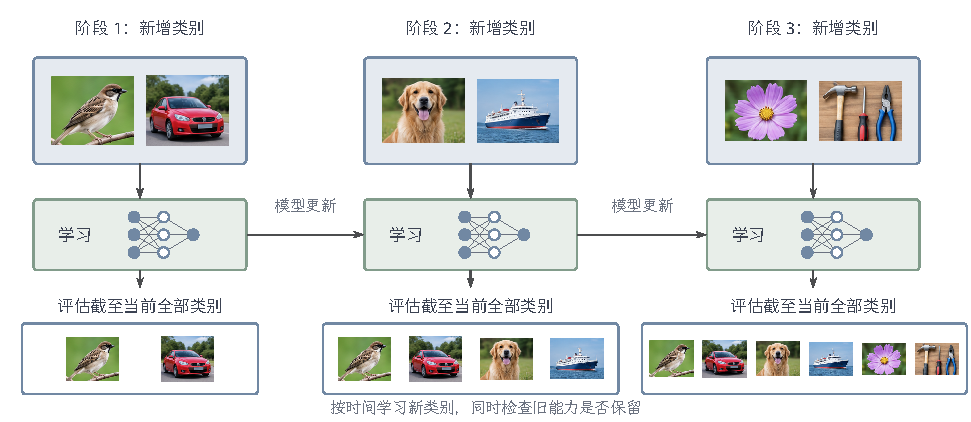
\includegraphics[width=164.600mm]{figures/03-foundations/01-basics/tikz/continual-learning/figure.pdf}
  \caption{持续学习的类别增量过程。不同类别的图像按阶段到来；每个阶段都要学习新增类别，并在截至当前出现过的全部类别上检查能力。横向箭头串接各阶段的模型更新，下方评价样本逐步纳入已经出现的类别，预测时不给阶段身份。样本图片为教学构造，模型框不对应精确记忆容量。}
  \label{fig:continual-learning-timeline}
\end{figure*}

\paragraph{任务增量学习}

如果学习的是一组彼此区分明确的任务——例如先学“识别猫和狗”，再学“识别汽车和卡车”——而预测时明确告知当前面对的是哪个任务，模型就可以切换到该任务对应的输出，这称为\term{任务增量学习}（task-incremental learning）。因为有任务身份作为提示，模型每次只需在当前任务的候选范围内判断，不必在所有历史类别中统一选择；它要解决的主要是“学新任务时不忘旧任务”，而选择范围扩大的问题被提示化解了。

\paragraph{领域增量学习}

还有一种常见情形：要识别的类别集合始终不变，变的只是输入数据的分布——比如同样是识别这些交通标志，训练和使用的场景从白天变成夜间。若输出含义保持不变、输入分布逐步改变，而且预测时不告知当前属于哪个领域，就称为\term{领域增量学习}（domain-incremental learning）。它既没有新类别要学，也没有任务提示可依赖，核心要求是在输入分布变化时维持原有输出的稳定。

\paragraph{三种设定的关系}

三种增量设定构成持续学习中常用的比较框架\scite{vandeven2019}，可以统一用交通标志的例子区分：标志种类陆续增加、且要在所有已见类别中选择，是类别增量；每次事先告知当前是哪一组识别任务，是任务增量；白天和夜间识别同一组标志、类别不变只是场景变化，是领域增量。它们改变的条件各不相同——类别增量扩大候选输出范围，任务增量改变预测时是否给出提示，领域增量保持输出含义而只改变输入分布，实际问题中这些条件还可能同时出现，所以报告成绩时必须说明是否给提示、在什么范围内预测。如果目标本就包含白天与夜间两种场景，只改善夜间而让白天失效，就不能算满足要求。

无论哪种设定，难度都还取决于三个现实条件：历史数据还能不能访问、任务边界有没有提示、在什么时间点评价。全部历史数据可用时，可以把合并历史记录重新训练作为比较基线，但仍要检查算力、响应时限以及新旧任务能否同时学好；只能保留少量旧样本时，复习手段就很受限。持续学习也能处理传感器、用户兴趣或任务本身的连续变化，但讨论时应先把这些条件讲清楚。

更新与维护的范围比持续学习更宽：还包括修正过时事实、按要求修改指定内容，或消除某些训练记录的影响。修改对象可以是参数、结构或外部记忆，也不以分布发生变化为前提。修改之后要分别验证四件事：目标内容是否改对、相关内容是否仍然一致、无关能力是否保留、系统之后是否还能继续学习，并记录版本和可恢复方式。

\subsection{多任务学习}
\label{sec:multi-task-learning}

如果几个相关任务的数据能在训练时同时访问，就可以让它们互相提供信息。街景识别和距离估计都可能需要物体边界这类共同信息。\term{多任务学习}（multi-task learning）通过共享表示或其他知识，同时学习多个任务的目标\scite{caruana1997}，使一个任务的反馈有机会帮助另一个任务；各自独立、互不联系地并行训练几个模型，则不会产生这种共享。多任务学习并不要求时间变化：任务集合可以固定，数据也可以事先收齐；各任务既可以共享同一份输入、使用不同标注，也可以各用各的数据集。它的定义核心是学习过程之间存在联系——一个任务的训练能够影响另一个任务。

街景中的\term{语义分割}（semantic segmentation）逐像素预测道路、车辆、建筑等类别，\term{深度估计}（depth estimation）估计像素所对应物体的距离。Kendall等人还加入区分物体个体的\term{实例分割}（instance segmentation），研究怎样平衡不同任务的反馈\scite{kendall2018}。平衡之所以成为问题，是因为共享部分只能沿一个方向更新。最简单的联合目标把各任务损失加权求和，$L(\bm{\theta})=\sum_{k}\lambda_kL_k(\bm{\theta})$，其中$L_k$是第$k$项任务的损失，$\lambda_k\geq 0$是它的权重。深度以米计、分割以类别概率计，两种损失的数值尺度本来就不同，若权重设置不当，数值大的一项就会主导共享参数的更新。Kendall等人的做法是根据各任务预测的不确定性自动学习这些权重，而不是手工逐一调试。

图~\ref{fig:multi-task-learning-process}仅展示语义与深度两项：同图经过共享模块，再分成两路预测，各路与自身标注比较，反馈共同调整共享部分。边界信息可能因此被两项任务复用，各自的预测要求却仍需保留。

多任务学习和持续学习的区别在于经验如何组织：训练期间如果各任务数据可以反复访问，即使交替更新，仍属于共同学习；如果经验按顺序到来、历史数据又无法完整访问，保留旧能力的问题就凸显出来，那是持续学习。单看任务数量区分不了二者。

\begin{figure*}[!htb]
  \centering
  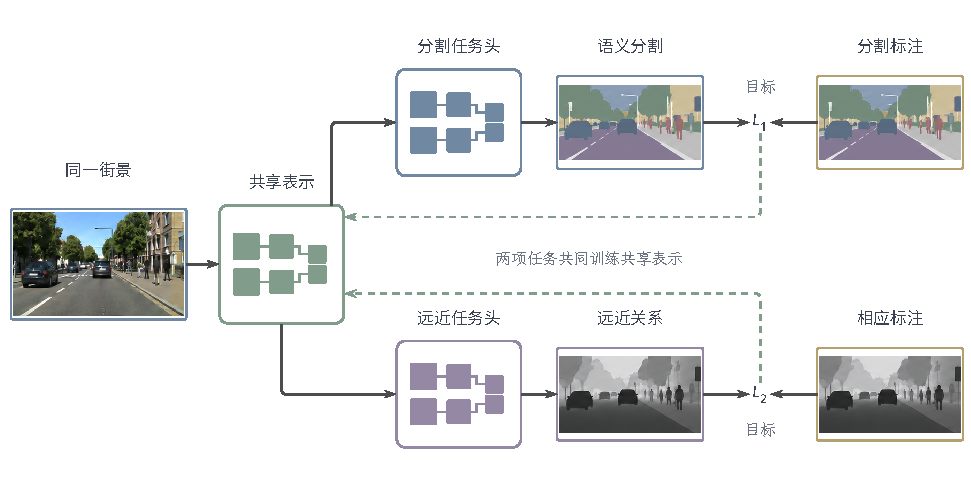
\includegraphics[width=164.600mm]{figures/03-foundations/01-basics/tikz/multi-task-learning/figure.pdf}
  \caption{多任务学习的过程示意。同一街景及不同任务的标注共同影响共享表示，系统分别输出
  语义区域和远近关系；两个结果都是概念示意，不是论文实验的实际输出。}
  \label{fig:multi-task-learning-process}
\end{figure*}

共享既可能带来收益，也可能带来损害：一个任务的更新可能干扰另一个任务，数据更多或更易学的任务还可能主导共享表示，把其他任务带偏。因此要分别报告每个任务的表现，再据此决定任务如何分组、共享哪些内容、采用什么结构、怎样合成联合目标，以及样本、更新和计算资源如何分配——一个汇总分数无法反映任务之间的干扰。

多任务学习关注多个任务在训练中怎样相互影响，多来源融合则考察怎样共同使用样本标注、模型预测输出、计算模块或模型参数。几个模型或模块分别训练好后，可以通过预测组合、结构连接、模型参数融合或\term{知识蒸馏}（knowledge distillation）共同使用；这些操作与多来源样本标注的融合发生在不同位置。蒸馏把教师模型的预测输出作为学生模型的训练目标，需要分别说明教师预测、学生训练样本及学生模型参数。融合还可以接入多任务训练，两者描述的关系可以同时成立；具体机制与条件可参考\BookChapterRef{chap:knowledge-fusion}{卷8《学习范式：知识的获取、演进与迁移》第6章“知识的融合”}。

\subsection{迁移学习}
\label{sec:transfer-learning}

已有的相关经验还可以直接帮助一个新的目标问题。\term{迁移学习}（transfer learning）明确区分来源与目标：把在来源任务上学到的表示、参数等知识用到目标任务上，以减少从头学习的需要。它既可以帮助标签稀少的目标任务，也可以用来加快训练或适应分布变化；但第一步永远是判断哪些来源知识对目标仍然有用。

以花卉识别为例，可以先复用在ImageNet上学到的图像表示，再用较少的花卉标签学习具体类别。来源知识提供了边缘、纹理、形状等通用基础，目标标签则负责规定不同花卉之间的细微差别，如图~\ref{fig:transfer-learning-process}所示。但通用来源不会自动给出花卉的分类标准：边缘、颜色、纹理可能可以共用，但足以区分汽车和动物的特征，未必能区分两种外形相近的花，这部分差异仍要靠目标标签来补足。

\begin{figure*}[!htb]
  \centering
  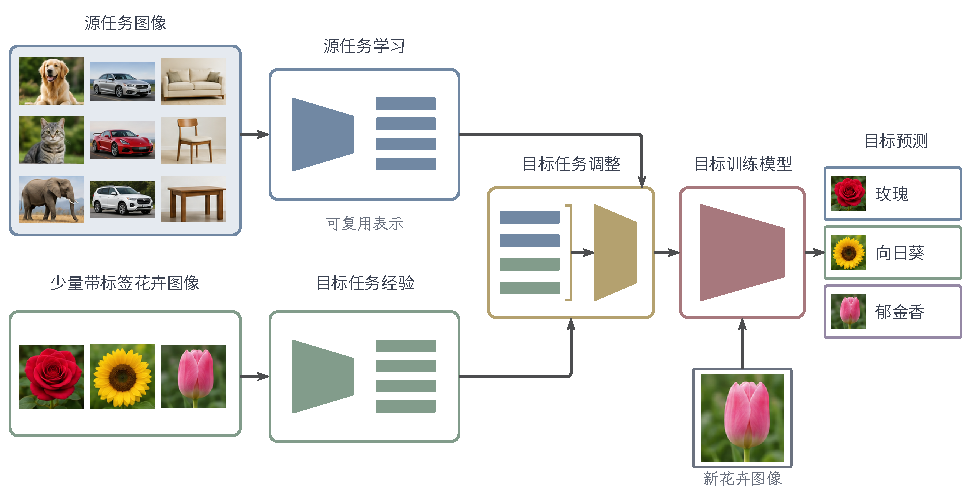
\includegraphics[width=164.600mm]{figures/03-foundations/01-basics/tikz/transfer-learning/figure.pdf}
  \caption{迁移学习的过程示意。通用图像任务形成可复用的表示，目标任务再用少量花卉标签调整
  这些知识，最后识别新的花卉照片；来源知识与目标数据共同决定结果。}
  \label{fig:transfer-learning-process}
\end{figure*}

哪些来源知识可以复用，与网络层次有关。图像网络的较早层通常提取边缘、颜色和局部纹理，越靠后的层越形成与原任务相关的组合特征。Yosinski等人的研究发现高层特征通常更依赖原任务：在其实验的任务划分下，来源与目标差异越大，冻结高层特征后目标分类的准确率相对“直接在目标上训练”的基线下降得越多\scite{yosinski2014}。但这一结论必须结合固定的目标评价样本和指标理解，不能推广成“高层一律不能复用”；究竟保留、调整哪些层，仍要针对具体目标检验。

复用方式主要有两种：以来源参数为起点、继续用目标数据调整，称为\term{微调}（fine-tuning）；也可以冻结已有表示，只训练目标侧的输出模块。选哪种取决于目标数据量、任务差异以及允许修改的范围。信息访问权限也会约束方案：来源方可能开放数据、参数、中间表示或模块，也可能只允许查询输出；目标侧可能提供标签、无标签输入、文字描述或后续反馈。因此应记录训练、模型选择和部署各阶段分别能使用哪些信息，相同的方法名称掩盖不了这些条件差异。

迁移不要求数据和任务同时改变：从通用分类转到花卉识别改变的是类别范围，白天到夜间可能类别不变、只改变输入分布，所以描述迁移时应逐项说明差异，而不能笼统说“换了一批数据”。

迁移还经常与其他范式同时出现，需要分清各自承担什么。迁移主要补充先前的知识，主动学习主要决定去获取哪些新标签，二者可以组合——先复用通用表示，再主动查询最需要确认的花卉照片，是否有帮助要同时检查来源相关性和新标签能否补足缺口。若深度表示帮助了语义分割而最终只关心后者，突出的是迁移；若两项任务共同训练、共享表示并分别评价，突出的是多任务。二者也可能重叠，迁移也可以通过共同训练实现，所以训练有没有先后并不是充分判据。与持续学习相比，迁移只要求目标任务表现好，持续学习还额外要求保住旧能力。

迁移未必有益。在相同的目标评价样本和相同可用信息下，如果复用来源知识后的指标反而不如从头训练（例如目标分类准确率更低），称为\term{负迁移}（negative transfer）。这个判断必须在目标任务上做出，来源数据规模多大、来源任务成绩多好都不能代替证据。决定是否复用还要比较标签或反馈需求，以及准备、适应、预测和存储各环节的成本；即使效果有提升，也不意味着每种成本口径都更划算。

当任务不变、只是拍摄环境改变时，还要弄清目标信息在什么时间点可用。本书用\term{域}（domain，也称领域）表示输入空间及其数据分布：\term{源域}（source domain）提供已有知识，\term{目标域}（target domain）是希望模型真正生效的环境。白天、雨天、夜间可能呈现不同的统计规律；域也不是由数据集名字唯一决定的，同一个数据集里可能包含多种环境。

如果夜间图片可以提前收集，就能用它们来调整只在白天训练过的模型。\term{领域自适应}（domain adaptation，亦称域适应或领域适应）根据可用的目标数据处理分布差异：目标域也有标签时是有监督设定；源域有标签、目标域只有输入时称为\term{无监督领域自适应}（unsupervised domain adaptation）。目标域没有标签，怎样让源域学到的分类器也适用于目标域？域对抗方法的思路是：如果白天和夜间图像经过模型得到的表示分布几乎一样，那么在白天表示上训练好的分类器，就有机会直接用于夜间表示。为此，它在训练分类器的同时训练一个“域判别器”，判别器努力从表示中分辨样本来自哪个域，提取表示的网络则努力让它分辨不出；两者对抗的结果，是在保留源域分类能力的同时缩小两个域的表示差异\scite{ganin2016}。但“无监督”只针对目标标签；表示分布对齐了，夜间的“汽车”也可能被对到白天的“卡车”附近，所以缩小域间差异并不自动保证目标任务正确。

更困难的情形是部署环境在训练时还不确定，目标数据完全不可用。\term{领域泛化}（domain generalization）只利用一个或多个源域，就要求模型在从未见过的目标域上工作\scite{muandet2013}，例如用若干城市白天、雨天的图像训练，之后直接预测此前没接触过的夜间图像。它比“同分布新样本”的评价多了一层环境差异，不能假定源域已经覆盖未来的所有变化。

“训练时不用目标域”这一限制也适用于调参、决定何时停止训练和选择模型：如果先看夜间图像上的成绩再挑配置，夜间数据就已经参与了学习，最终分数会高估真正未知环境中的表现。那么不看目标域，又该怎样选择配置？一种常用做法是从多个已知源域中整体留出一个（例如雨天），只用其余源域训练，再看模型在留出域上的表现，以此模拟“换到新环境”。它不同于在同一域内随机留出若干样本，因为后者只检验同分布的新样本；但留出的雨天也只能模拟某一类环境变化，未必代表夜间。Gulrajani与Lopez-Paz专门研究了这类选择方式对评价结论的影响\scite{gulrajani2021}。

在本章的标准设定中，目标数据只用于最终检验。用固定参数对夜间图像计算预测并不改变模型；只有利用这些输入调整了参数或统计量，才算发生了适应，那属于后面介绍的设定。

多个源域之间稳定不变的物体形状，可能帮助模型减少对背景的依赖；但“源域之间稳定”不等于“对任意目标域都稳定”，增加源域数量也不必然改善目标表现。如果未来的输入或标签规律任意改变，过去的经验无法保证成功。领域泛化依赖的仍是来源与目标之间可利用的联系，其学习条件将在第~\ref{sec:domain-generalization}节进一步说明。

部署之后如果能持续看到目标输入，就又有了适应的机会。\term{测试时适应}（test-time adaptation）按事先约定，利用测试或部署阶段的数据更新参数或统计量，常见设定下没有目标标签。Tent用测试输入和模型自己的预测更新部分参数，通过降低预测分布的熵让类别概率更集中\scite{wang2021tent}。熵衡量概率分布的分散程度：模型对十个类别各给$0.1$时熵最大，把概率几乎全给一个类别时熵接近零。这一做法依据的观察是，在分布变化下熵较低的预测往往错误也较少；但这只是统计上的关联，模型自信同样可能伴随着错误，这类更新可能把错误放大。评价时必须规定输入的可见范围、更新时序以及跨样本是否保留状态。

表~\ref{tab:domain-transfer-settings}按“目标域信息在哪个阶段可用”对照四种设定。如果训练阶段按领域泛化准备、部署后又继续适应，系统就同时涉及两套条件；报告时应明确说明发生了更新，不能把适应后的结果当作固定模型的直接泛化能力。

\begin{table*}[htbp]
  \centering
  \small
  \begin{tabularx}{\linewidth}{@{}lXX@{}}
    \toprule
    \textbf{设定} & \textbf{可用的目标域信息} & \textbf{关键条件} \\
    \midrule
    有监督领域自适应 & 适应时已有目标域带标签样本 & 用目标监督调整模型，另留样本评价 \\
    无监督领域自适应 & 适应时已有目标域无标签输入 & 源域标签与目标域输入共同参与学习 \\
    领域泛化 & 训练及模型选择时均无目标域数据 & 本章标准设定在目标域直接预测，不更新模型 \\
    测试时适应 & 测试或部署时利用目标输入；常见设定无标签 & 按约定更新参数或统计量，并说明数据与时序限制 \\
    \bottomrule
  \end{tabularx}
  \caption{目标域数据的可用性区分领域自适应、领域泛化与测试时适应。前两行区分目标监督条件，
  最后一行强调适应发生的阶段；它们不是完全互斥的分类。}
  \label{tab:domain-transfer-settings}
\end{table*}

目标域有多少标签，构成另一项条件。花卉分类中如果每个类别只有极少几个带标签样本，本书称为\term{少样本学习}（few-shot learning）；如果目标类别的带标签样本一个都没有，只能借助先前知识和类别描述等信息，则称为\term{零样本学习}（zero-shot learning）。二者限定的是目标侧的资源多少，并不规定来源知识如何获得、如何迁移。

要让类别文字直接参与识别，模型必须先建立图像与文字之间的联系。CLIP同时学习图像表示和文本表示，使配对图文的匹配得分高于同一批中不配对的组合\scite{radford2021}。它沿用了第~\ref{sec:contrastive-learning}节的关系匹配目标，但比较的双方变成了图像和文字，学到的经验也包括“视觉内容如何对应语言描述”。

使用时，可以把候选类别写成“a photo of a cat”（一张猫的照片）、“a photo of a dog”（一张狗的照片）这样的描述，让新图像分别与各描述比较匹配得分、取最高者。这样无需为目标类别提供任何新的带标签训练图，因此属于零样本分类。但“零”只表示这部分数据为零：模型仍依赖大规模已有的图文配对经验，也不能据此断言预训练数据里没有相关概念。零样本与领域泛化的限制方向也不同：前者限制目标类别的标签，后者限制目标域数据在训练和选择中的使用。新类别可以出现在熟悉的环境里，新环境也可能包含源域已有的类别，两个条件要分别判断。

\subsection{元学习}
\label{sec:meta-learning}

考虑一个要反复识别新字符的系统：每次遇到一套新字符，都只有寥寥几个示例，但这样的“适应任务”会反复出现。这时可以提前练习“怎样快速适应”——把许多小任务当作学习经历，用每次适应之后的表现反过来改进下一次学习，而不仅仅是学一个固定表示。这种从一组任务的学习经历中改进后续学习的方法，称为\term{元学习}（meta-learning）。它可以服务于少样本适应，也可以关注适应的速度或稳健性\scite{hospedales2022}。“学习如何学习”概括的是跨任务经验的作用，但实际系统仍要预先规定模型、目标和更新方式，并非凭空获得学习能力。

仍以新字符识别为例：可以让模型每次都从同一组起始参数出发，用少量示例做适应，再用同一任务的另一批样本检查预测损失。\term{模型无关元学习}（model-agnostic meta-learning, MAML）就用这些适应后的检查损失来更新起始参数，使模型从这个起点出发、经过少量样本适应后就能取得较低的损失\scite{finn2017}。

以只做一步梯度适应的情形为例，可以把这两层更新写出来。记共同起点为$\bm{\theta}$，任务$\tau$的适应样本上的损失为$L^{\mathrm{adapt}}_{\tau}$，同任务另一批检查样本上的损失为$L_{\tau}$，$\alpha,\beta>0$为两层的步长。任务内适应从起点走一步：
\begin{equation}
  \bm{\theta}'_{\tau}=\bm{\theta}-\alpha\nabla_{\bm{\theta}}L^{\mathrm{adapt}}_{\tau}(\bm{\theta});
  \label{eq:maml-inner-overview}
\end{equation}
跨任务更新则按适应后参数的检查损失调整起点：
\begin{equation}
  \bm{\theta}\leftarrow\bm{\theta}-\beta\nabla_{\bm{\theta}}\sum_{\tau}L_{\tau}(\bm{\theta}'_{\tau}).
  \label{eq:maml-outer-overview}
\end{equation}
第二式的关键在于，$L_{\tau}$在适应后的参数$\bm{\theta}'_{\tau}$处计算，而$\bm{\theta}'_{\tau}$又由第一式依赖于$\bm{\theta}$，所以梯度要穿过适应这一步传回起点。换句话说，评价对象变了：不再是起点本身的损失，而是“从这个起点适应一步之后”在新样本上的损失。

MAML的Omniglot实验把少数几个手写字符类别组成一项任务。每项任务都从共同参数出发、用少量标签适应，再用同任务的另一批样本检查对新写法的识别；这些检查结果汇总成元学习目标，用来更新共同起点，之后再换下一组任务继续练习。这个准备阶段称为\term{元训练}（meta-training），被反复优化的是“以后适应得好不好”。

图~\ref{fig:meta-learning-process}中需要注意两批检查数据的区别：任务内的检查样本虽然没用于该次少样本适应，却通过元学习目标参与了起始参数的更新，仍属于元训练；最终评价则使用完全没参加过元训练的新任务（在字符实验中对应新类别），只考察用少量新示例适应之后的效果。两类检查数据不能混用。

\begin{figure*}[!t]
  \centering
  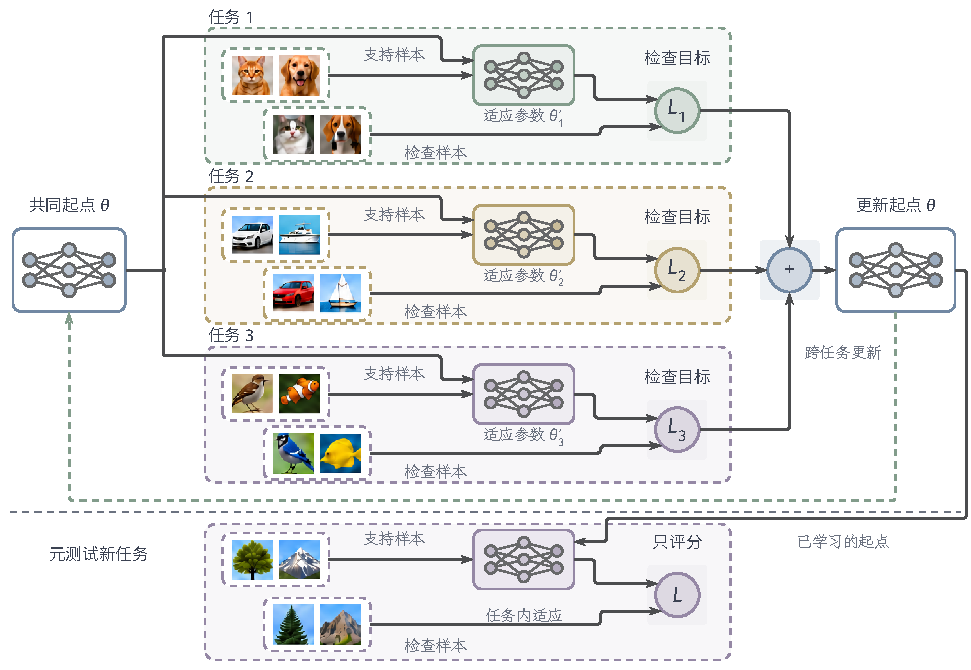
\includegraphics[width=164.600mm]{figures/03-foundations/01-basics/tikz/meta-learning/figure.pdf}
  \caption{任务内适应与跨任务更新。元训练任务从共同起点$\bm{\theta}$出发，用任务内适应样本得到参数$\bm{\theta}'_{\tau}$，再汇总另一批检查样本上的损失$L_{\tau}$来更新起点；两批样本都参与元训练。未参加元训练的新任务只用少量适应样本调整参数，最终检查评分不回传共同起点。任务与图像样本为教学构造，不是Omniglot原始样本。}
  \label{fig:meta-learning-process}
\end{figure*}

普通预训练同样能得到一组可迁移的参数，它和元学习的差别在准备阶段优化的目标。如果把旧字符合并起来做普通监督分类，反馈来自来源任务上的识别误差；MAML则把数据组织成一个个“少样本任务”，先适应、再检查，反馈来自适应后在该任务新样本上的表现。即使两者使用的旧字符完全一样多，一个起点是为“来源识别”优化的，另一个是为“少量示例后的学习效果”优化的；使用时都可能载入参数再做少量调整，所以只有追溯准备阶段才看得出区别。

总的来说，迁移关注来源如何帮助目标，元学习关注历史任务如何改进学习过程本身；把元学习得到的起点用于新任务，也可以看成一种迁移。这里的比较只针对普通监督预训练和MAML，不能据此把两类范式看成互斥的。

还要澄清：少样本描述的只是数据条件，普通迁移等方法同样能处理\scite{wang2020}。元学习能否带来收益，取决于练习任务与未来任务是否相关：差异过大时，练出来的适应方式可能根本用不上。而新任务只给几个示例，也不意味着准备阶段只见过几条数据——它背后往往需要大量历史任务。

示例还有一种用法：不更新任何参数，只把它们放进预测输入。给语言模型几条“评论—情感标签”的例子，再给一条新评论让它作答，模型参数全程不变，这称为\term{上下文学习}（in-context learning），GPT-3的少样本实验采用的就是这种方式\scite{brown2020}。所以同样是“给几个新示例”，要区分它们是进入了输入上下文还是触发了参数更新；模型能照着示例作答，也不足以证明它曾接受过以“适应能力”为目标的元训练。

反过来说，训练时涉及多个任务也不一定就是元学习。街景多任务学习的目标是把已有的分割、深度等任务做好；少样本元学习则借历史任务练习适应、再在没见过的任务上评价。区分二者时，任务承担的用途和最终评价对象比任务数量更说明问题。

\subsection{数据与任务变化下的比较}
\label{sec:knowledge-evolution-comparison}

表~\ref{tab:knowledge-evolution-comparison}从数据、任务组织和评价三个角度汇总这四种范式。多任务学习的任务集合可以固定；持续学习可以只面对同一任务下的数据分布变化；迁移学习和元学习都能处理新任务，但元学习还要进一步追问准备阶段是否真正改进了学习过程。除了变化本身，变化发生的时间、知识服务于谁、对能力保留有什么要求，都应一起报告。

\begin{table*}[htbp]
  \centering
  \small
  \begin{tabularx}{\linewidth}{@{}lXXX@{}}
    \toprule
    \textbf{范式} & \textbf{数据怎样变化} & \textbf{任务怎样组织} & \textbf{主要评价要求} \\
    \midrule
    持续学习 & 经验顺序到来，分布可能变化；旧数据访问常受限 & 任务可以不变，也可增加类别或依次出现新任务 & 学习新内容，同时保留所需旧能力 \\
    多任务学习 & 各任务可共享输入，也可使用不同数据集；不要求随时间变化 & 一组相关任务共同学习，任务集合可以固定 & 分别检查各任务表现与共享带来的影响 \\
    迁移学习 & 来源与目标的分布可以不同 & 区分来源与目标；目标任务可相同或不同 & 来源知识是否帮助目标任务 \\
    元学习 & 用训练任务积累学习经验，再以新任务数据考察适应 & 跨任务改进学习过程；本节以少样本适应为例 & 在给定适应数据和预算下学得怎样 \\
    \bottomrule
  \end{tabularx}
  \caption{从数据、任务及评价要求比较知识的演进与迁移。各行描述本节的典型设定，
  不是由“变或不变”唯一确定的互斥类别。}
  \label{tab:knowledge-evolution-comparison}
\end{table*}

用同一个道路场景就能把四种要求区分开：只问白天学到的知识能否帮助夜间识别，突出的是迁移；按时间顺序接触不同环境、同时要求保住白天能力，加入的是持续学习；同时训练物体识别和距离估计，体现的是多任务；先用大量历史场景练习“如何用少量示例快速适应”、再到新场景检验，体现的是元学习。新数据或多个任务可能出现在各种设定中，真正把它们区分开的是知识的组织方式和评价要求。

跨域问题还应按信息可用的时机细分：夜间数据在训练前就能参与学习，是领域自适应；训练和模型选择阶段都见不到目标、只能直接预测，是领域泛化；部署之后才用目标输入更新模型，是测试时适应。所以除了“变化了什么”，还必须说清“哪些信息在什么时候可用”。

这些方式还可以沿时间或任务串联起来：多任务学到的表示可以成为迁移的起点，元学习练出的适应方式也可以用于连续到来的任务。组合是否可行，仍要检查所需数据此刻能否访问，以及评价是否覆盖了真正需要获得和保留的能力。

因此评价不能只剩一个当前任务的平均分：目标适应要报告效果与代价，持续更新要同时检查新知识、历史能力和后续可学性，指定修改和能力融合还要检查修改范围、来源能力和组合结果。人工、计算、存储和维护成本也应分别呈现，在没有换算依据时，不宜强行压成一个数字。

\section{其他范式}
\label{sec:other-learning-settings}

反馈形式和目标确定之后，学习还会受到另外两类条件限制：经验可能逐条到来，从而限制预测和更新的时序；数据也可能分散在不同设备上，从而限制存放方式和协作形式。本节用在线学习和联邦学习说明这两种条件。它们都可以叠加在前面介绍的任何范式之上，所以学习范式两卷没有为它们设立并列部分：在线学习的时序问题归入交互与更新，联邦学习的协作问题归入相应专题，具体的工程实现则由系统卷展开。

\subsection{在线学习}
\label{sec:online-learning}

当经验持续不断到来时，学习者可以先用当前模型作出预测或决策，等后续反馈到达后再更新，然后处理下一个输入——这种时序安排称为\term{在线学习}（online learning）。与之相对的\term{批量学习}（batch learning）则是先拿到一整批数据完成训练，再使用训练好的模型。两者的区别在于经验进入更新的时间安排。

广告系统是典型例子：先根据广告内容和展示场景预测用户是否点击，之后观察真实点击结果并更新模型，如此往复\scite{mcmahan2013}。点击结果提供的是监督目标，“在线”规定的只是目标到达和使用的时序；反馈可以延迟，更新也可以攒成小批次进行。还要注意，系统联网或实时响应本身并不构成在线学习——如果新反馈从不改变模型，那只是在持续地做预测。

图~\ref{fig:online-feedback-order}对照了两种系统：一种按“先预测、后更新”的顺序使用反馈，另一种始终用固定参数预测。在线评价必须保存“反馈尚未到达时”作出的预测，之后的更新只能作用于后续输入；如果用更新后的模型重算旧样本，就无法还原当时的真实表现。

\begin{figure*}[!tbp]
  \centering
  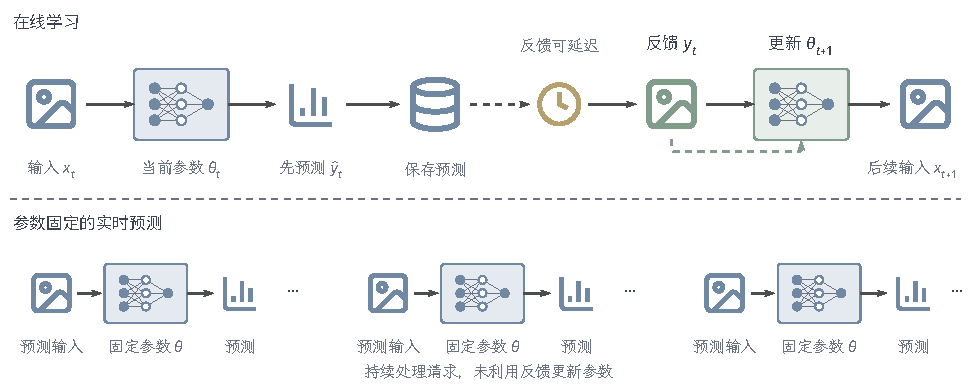
\includegraphics[width=164.600mm]{figures/03-foundations/01-basics/tikz/online-feedback-order/figure.pdf}
  \caption{在线学习先用当前模型预测并保存此时尚未看到答案的结果，反馈可以延迟或按小批次到达，随后更新只作用于后续输入。下方对照只用固定参数持续响应的实时预测；请求持续到来本身不构成在线学习。}
  \label{fig:online-feedback-order}
\end{figure*}

在线学习和持续学习可以重叠，但限定的条件不同。即使数据始终同分布，也可以逐条预测、逐条更新，所以在线并不要求任务变化，也不专门要求保留旧任务；持续学习关注的是长期适应和能力保留，更新既可以在线进行也可以按阶段批量进行。如果一个系统既逐次学习反馈、又在评价旧能力，它就同时符合两种描述。

在线学习之所以常被用于长期运行的系统，一个原因是数据的统计规律会随时间改变，这称为\term{分布漂移}（distribution drift）。把输入记为$\bm{x}$、目标记为$y$，联合分布可以拆成$p(\bm{x},y)=p(\bm{x})\,p(y\mid\bm{x})$，两部分都可能变化。\term{概念漂移}（concept drift）在本书中专指后一部分$p(y\mid\bm{x})$的变化，即给定输入后目标规律改变，例如同样的广告和用户特征不再产生原来的点击倾向；如果只是用户或广告的构成比例变了，即$p(\bm{x})$变化而$p(y\mid\bm{x})$不变，则称为输入分布漂移，对应后文所说的协变量偏移（covariate shift）。两类漂移可能同时出现，前者意味着旧答案本身过时，后者只意味着各类输入出现的频率改变，识别方式和调整手段因而不同，常见做法包括检测变化或调整历史经验的权重\scite{bifet2007}。在线学习只提供了利用新反馈的时序，并不能保证克服漂移，还会受到反馈延迟和样本不足的限制；变化各部分的形式化区分见第~\ref{sec:distribution-shift}节。

除了遵循前述“先预测、后更新”的信息顺序，在线评价还要报告反馈延迟多久、保留多少历史数据、更新预算多大：这些条件决定了模型在何时、依据多少经验发生改变。

\subsection{联邦学习}
\label{sec:federated-learning}

手机键盘需要大量多样的用词经验才能预测下一个词，但单台设备只有机主的一小部分记录，而且原始文本不便集中上传。这里要解决的是“如何共同利用分散的经验”，而不一定是总样本量不够。\term{联邦学习}（federated learning）给出了一种保留本地数据的协作安排：各设备或机构的数据不出本地，只通过交换模型相关信息来共同训练。手机键盘研究就在设备端学习下一词预测，再汇总各方结果改进共享模型\scite{hard2018}。这里下一词目标由原文本构造，属于自监督信号；联邦则规定各方经验如何协作，二者限定的是不同方面。

在有中心协调的方案中，一轮协作如下进行：中心先把当前共享模型下发给各方，各方从同一模型出发、用自己的本地数据训练，再上传训练后的参数。\term{联邦平均}（federated averaging, FedAvg）按各方样本量加权汇总这些参数\scite{mcmahan2017}。记本轮参与方集合为$I_t$，第$i$方的本地训练样本为$D_i$、记录数为$n_i=|D_i|$，并要求参与方总样本量大于零，则总样本量与聚合参数写为
\begin{equation}
  n=\sum_{i\in I_t}n_i,\qquad
  \bm{\theta}^{(t+1)}
  =\sum_{i\in I_t}\frac{n_i}{n}\bm{\theta}_i^{(t+1)}.
  \label{eq:fedavg-overview}
\end{equation}
其中$\bm{\theta}^{(t)}$是第$t$轮下发的共享参数，$\bm{\theta}_i^{(t+1)}$是第$i$方从它出发完成本地训练后的参数。各方权重$n_i/n$之和为1，所以结果是本地参数的加权平均，记录更多的参与方占比更高。例如两台设备分别有300条和100条记录，权重就是$3/4$与$1/4$。按记录数加权的用意，是让汇总结果接近“把所有记录放在一起”时各条记录的贡献比例。

但这只是近似。每台设备在本地走了多步，各方的参数沿着各自数据的方向漂移，平均之后，各条记录对最终参数的实际影响未必相同，结果也不保证等于集中训练所得的参数；各方数据分布差异越大，这种偏离越值得检查。公式也可以等价地写成对各方参数改变量$\bm{\theta}_i^{(t+1)}-\bm{\theta}^{(t)}$的加权平均；若改用其他权重，则需说明理由。图~\ref{fig:federated-learning-process}展示下发、本地学习和汇总的循环。

\begin{figure*}[htbp]
  \centering
  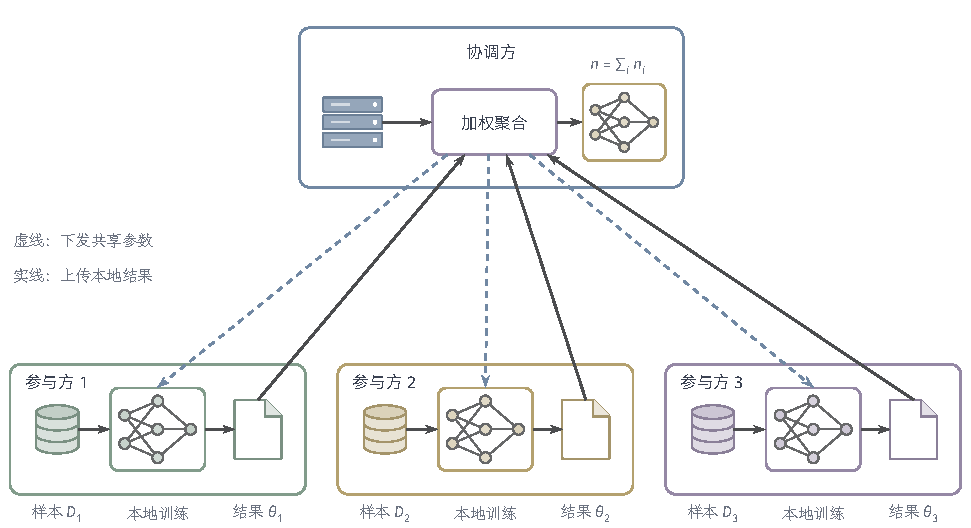
\includegraphics[width=164.600mm]{figures/03-foundations/01-basics/tikz/federated-learning/figure.pdf}
  \caption{中心协调式联邦学习的一轮通信。协调方向三个示意参与方下发同一组共享参数$\bm{\theta}^{(t)}$；各方使用自己的本地训练样本$D_i$训练，得到本地参数$\bm{\theta}_i^{(t+1)}$并上传。协调方按正文所述的训练记录数权重形成下一版本$\bm{\theta}^{(t+1)}$，下一轮再统一下发。参与方数量为教学示意；原始记录留在本地，但模型更新仍可能泄露信息，联邦组织方式本身不提供隐私保证。}
  \label{fig:federated-learning-process}
\end{figure*}

联邦协作还会遇到数据量、算力和设备在线状态不一致的问题，也要承担反复下发、上传模型的通信成本。更要强调：原始记录虽然留在本地，但模型更新仍可能泄露其中信息，隐私保护还需要额外机制（例如限制单设备更新的可见性）；聚合过程和系统实现都需要专门核查，隐私机制的系统讨论见第\ref{part:trustworthy-ml}部分。

共享模型也未必适合每个用户：设备可以在共享知识基础上做本地化适应，也可以用多任务方式保留参与方之间的差异；当用户习惯随时间改变时，还要结合持续学习检查旧能力。分散协作、个体适应与旧能力保留，往往共同构成一项系统任务。

\FloatBarrier
\section{范式的组合}
\label{sec:combining-learning-paradigms}

各种范式分别限定反馈形式、标签利用方式、知识复用以及时序和协作环境，而同一个系统完全可以在不同阶段组合它们，也可以在同一阶段使用多种信号。说明一个组合系统时，应该逐步追踪数据、目标和反馈的流向，讲清每一阶段把什么知识传给了下一步，才能看出每种设定各自承担什么职责。

自监督文本预训练之后再接任务标签做监督学习，是典型的分阶段组合：前者积累通用表示，后者把表示调整到分类、问答等具体用途。半监督学习则在同一个目标任务中同时使用标签和无标签输入，还可以额外加入自监督目标。两者都使用了多种信号，但阶段划分和任务组织方式不同，这一差别不能省略。

AlphaGo（2016）的训练主线是两阶段组合的经典案例：先利用专家棋谱中的“局面—落子”配对训练策略网络，再通过自我对弈、按胜负继续改进\scite{silver2016}。传入第二阶段的是一个初始策略，而反馈来源从“专家怎样下”变成了“对局结果如何”，如图~\ref{fig:paradigm-combination-alphago}所示（完整系统还包括价值网络和搜索等组件）。自我对弈依据的是胜负奖励，属于强化学习，不能因为有“自我”二字就误认为自监督。

\begin{figure*}[!tbp]
  \centering
  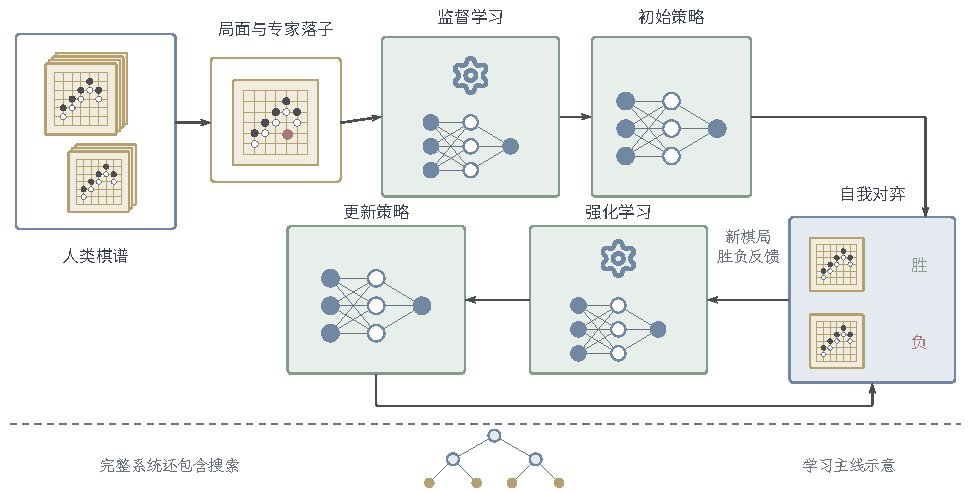
\includegraphics[width=164.600mm]{figures/03-foundations/01-basics/tikz/alphago-paradigm-combination/figure.pdf}
  \caption{AlphaGo学习主线的简化示意。人类棋谱为监督学习阶段提供局面与专家落子；得到初始策略后，
  自我对弈产生新棋局与胜负反馈，用于强化学习阶段。完整系统还包含价值网络与搜索等组件。}
  \label{fig:paradigm-combination-alphago}
\end{figure*}

当行为难以逐步打分时，人往往仍能比较两段行为的好坏。\term{偏好学习}（preference learning）利用的就是这种相对判断；与强化学习组合时，先请人在两段行为片段中选出更符合要求的一段，据此训练一个评价模型，再用学出的奖励训练智能体，相关研究已用于Atari游戏和模拟机器人\scite{christiano2017}。这里人提供的是“好坏比较”，而不是每一步的正确动作；评价模型把比较转成奖励，策略再依据奖励学习。

用一个假想的多机构花卉识别系统，可以看清更多环节如何各司其职：各机构保留自己的照片、以联邦方式协作；本地无标签照片生成不同视图，通过自监督对比目标学习表示；系统还可以主动请专家标注一部分照片，再把其余无标签照片用于半监督训练；学到的通用表示可以迁移到新机构，而新物种陆续出现时还要用持续学习检查旧能力。其中联邦规定协作方式、自监督规定信号来源、对比规定目标构造，三种描述同时成立却不能互相替代。这个情景只用于解释组合方式，实际系统按需选用其中环节即可；需要记住的是：挑选标签替代不了目标学习，协作也不会自动消除来源差异、标注错误或旧能力遗忘。

\section{本章小结}
\label{sec:machine-learning-paradigms-summary}

本章自始至终围绕“经验和反馈”来辨认范式，而不是按模型名称分类：任务规定目标，模型表达候选规律，范式组织学习所依据的经验。开头的三个问题分别有了答案。

第一个问题是训练依据从哪里来。监督学习依赖输入与目标的配对，无监督学习从数据中发现结构或分布，强化学习依据行动后果的奖励改进决策。辨认一个实际系统时，要先追溯它究竟得到了什么经验，再检查训练和评价是在什么条件下进行的。

第二个问题是标签不足时怎么办。可以让无标签输入直接参与目标任务（半监督），从数据自身构造新目标（自监督），接受并修正质量不完善的监督（弱监督），或者主动挑选最值得标注的样本获取答案（主动学习）；对比学习则提供了利用样本间关系的具体方式。这些方法都建立在信号可靠且与任务相关的前提上，减少人工标签并不自动带来能力提升；来自人工、规则、模型和数据的候选知识，都必须经过对齐、融合、评估和修正才能使用。

第三个问题是数据和任务变化以后怎么办。持续学习强调顺序适应与旧能力保留，多任务学习强调共同训练中的知识共享，迁移学习强调来源知识对目标的帮助，元学习强调历史任务对后续学习过程本身的改进；目标信息在训练、选择还是部署阶段可用，又进一步区分了领域自适应、领域泛化和测试时适应。对已有表示、参数、模块、记忆和学习策略的复用、更新与整合，都要分别检查效果以及样本、计算、存储和维护成本，在明确的预算下取舍。在线学习和联邦学习则在这些范式之上，分别限定更新时序和协作方式。组合多种范式时，应逐步说明数据、反馈、任务关系和信息权限，再评价系统真正需要获得和保留的能力。

\paragraph{扩展阅读}

继续学习交互决策可读Sutton与Barto的教材；弱监督与元学习可分别参阅相关综述；联邦平均的原始论文提供了分散协作的具体入口\scite{sutton2018,zhou2018,hospedales2022,mcmahan2017}。结合第~\ref{chap:machine-learning-models}章，我们已经有了“模型如何表示规律”和“学习如何利用经验”两个基本框架。第\ref{part:learning-theory}部分将在给定经验、学习目标和比较标准下，研究能否从有限样本学到所需结果；第\ref{part:trustworthy-ml}部分则检查这些方法进入实际流程后的可靠性、鲁棒性、公平、隐私、安全与处置要求。交互决策、训练依据获取和已有知识利用还需结合专题继续深入，协作部署则还要检查具体的系统实现。
